\documentclass[12pt, letterpaper]{article} % Sets the font size to 12pt and paper size to letter

\usepackage[margin=1in]{geometry} % Sets the margins to 1 inch all around
\usepackage{setspace} % Allows for double spacing and setting line spacing
\setlength{\marginparwidth}{2cm}

\usepackage{graphicx}
\usepackage[utf8]{inputenc}

\usepackage{amsmath}
\usepackage{amssymb}
\usepackage{floatpag}
\usepackage{bm}
\usepackage{algorithm2e}
\usepackage{csquotes}
\usepackage[T1]{fontenc}
\usepackage{hyperref}
\usepackage{textcomp} % provide symbols
\usepackage{todonotes}
\usepackage{xr}
\usepackage{pdflscape}
\usepackage{afterpage}
\usepackage{caption}
\usepackage{numprint}
% \usepackage{microtype}
\usepackage[USenglish]{babel}
\usepackage[nameinlink]{cleveref}
\usepackage[backend=biber,style=apa,natbib=true]{biblatex} % Load biblatex with the desired settings
\addbibresource{references.bib}
\addbibresource{refs-custom.bib}
% no URLs
\AtEveryBibitem{
  \clearfield{url}
  \clearfield{doi}
}

\captionsetup{font=footnotesize} % Adjust the caption font size as necessary for readability

% \usepackage{lineno} % Include the package for line numbering
% \linenumbers % Activates line numbering for the document

% Diagrams
\usepackage{tikz}
\usetikzlibrary{arrows,positioning,automata,fit}

% Macros for common abbreviations to get the spacing right
% See: https://stackoverflow.com/questions/3282319/correct-way-to-define-macros-etc-ie-in-latex
\usepackage{xspace}
\makeatletter
\DeclareRobustCommand\onedot{\futurelet\@let@token\@onedot}
\def\@onedot{\ifx\@let@token.\else.\null\fi\xspace}
\def\eg{e.g\onedot} \def\Eg{\emph{E.g}\onedot}
\def\ie{i.e\onedot} \def\Ie{\emph{I.e}\onedot}
\def\cf{c.f\onedot} \def\Cf{\emph{C.f}\onedot}
\def\etc{etc\onedot} \def\vs{\emph{vs}\onedot}
\def\wrt{w.r.t\onedot} \def\dof{d.o.f\onedot}
\def\etal{et al\onedot}
\makeatother

% Generic maths commands
\def\reals{\mathbb{R}}
\def\nats{\mathbb{N}}
\def\sampSpace{\mathcal{X}}
\def\dist{\sim}
\DeclareMathOperator{\E}{\mathbb{E}}
\DeclareMathOperator{\V}{\mathbb{V}}
\DeclareMathOperator{\I}{\mathbb{I}}
\DeclareMathOperator{\prob}{\mathbb{P}}
\DeclareMathOperator{\p}{\pi}
\DeclareMathOperator{\var}{\mathbb{V}}
\DeclareMathOperator{\indicator}{\mathbb{I}}
\DeclareMathOperator{\cov}{Cov}
\DeclareMathOperator{\cor}{Cor}
\DeclareMathOperator{\logit}{logit}
\DeclareMathOperator{\Ber}{Bernoulli}
\DeclareMathOperator{\Bin}{Binomial}
\DeclareMathOperator{\Poi}{Poisson}
\DeclareMathOperator{\BetaDist}{Beta}
\DeclareMathOperator{\Exponential}{Exponential}
\DeclareMathOperator{\NBr}{NegBin}
\newcommand{\NBc}{\NBr_{c}}
\newcommand{\NBs}{\NBr_{s}}
\DeclareMathOperator{\BB}{BetaBin}
\DeclareMathOperator{\GamDist}{Gamma}
\DeclareMathOperator{\MN}{Multinomial}
\DeclareMathOperator{\N}{N}
\DeclareMathOperator{\LN}{LN}
\DeclareMathOperator{\LKJ}{LKJ}
\DeclareMathOperator{\expit}{expit}
\newcommand\matr{\bm}
\newcommand\set{\mathcal}
\renewcommand{\vec}{\bm}
\newcommand{\ssep}{:}

% Thesis-specific maths commands
\newcommand{\dmax}{d_\text{max}}
\newcommand{\psens}{p_\text{sens}}
\newcommand{\ntot}{n_\text{tot}}
\newcommand{\ndet}{n_\text{d}}
\newcommand{\nnodet}{n_\text{u}}
\newcommand{\pnodet}{p_\text{u}}
\newcommand{\Npop}{N_\text{pop}}
\newcommand{\Ncis}{N_\text{CIS}}
\newcommand{\ncis}{\vec{n_\text{CIS}}}
\newcommand{\na}{\vec{n_\text{a}}}
\newcommand{\pcis}{\vec{p_\text{CIS}}}
\newcommand{\sched}{\mathbb{T}}
\newcommand{\nsched}{n_{\sched}}
\newcommand{\rate}{\mathfrak{R}}
\newcommand{\R}{\mathcal{R}_{0}}
\renewcommand{\Re}{\mathcal{R}_{e}(t)}
\newcommand{\Rc}{\mathcal{R}_{c}(t)}
\newcommand{\vlod}{v_\text{lod}}
\newcommand{\inform}{{_{\text{inform}}}}


\begin{document}

\title{Estimating length of SARS-CoV-2 from doubly interval censored data with missed infections}
\author{Blake, TBC, Birrell, De Angelis}
% \date{\today}
\maketitle

\begin{abstract}
Abstract goes here.
\end{abstract}

\textbf{Notes / thoughts on current version}
\begin{itemize}
    \item Some of the derivations can be moved to a supplement (cut 2--3 pages).
    \item Need to rearranage the ATACCC stuff --- add some details of what I did (thesis ch 4) and move stuff from prior info section into supplement.
    \item Probably don't need some of the figures (maybe 5--8)?
    \item Should the sensitivity analyses (figs 13/14 be in the main text)?
    \item The above changes make this about the right length.
\end{itemize}

The \textbf{format requirements from JASA} are at \url{https://www.tandfonline.com/journals/uasa20}.
The most important parts are reproduced here.
\begin{itemize}
    \item Should be written with the following elements in the following order: title page; author footnote; abstract; keywords; article text (table(s); figures); acknowledgments; appendices; references
    \item Should be no more than 35 pages, including the abstract, figures, tables, and references. Appendices, proofs, and other supporting material should be placed in a separate supplement file (anonymized for review)
    \item Should contain an unstructured abstract of 200 words.
    \item Should contain between 3 and 5 keywords. Read making your article more discoverable, including information on choosing a title and search engine optimization.
    \item JASA requires that all papers be formatted for 8 1/2 x 11-inch paper, one side only.
    \item 12 point, double-spaced font (which we define as 26 lines of text per page)
    \item the average JASA paper is about 30 manuscript pages (with the above page format and including all appendices, references, tables, and figures), and it is very uncommon for papers much longer than about 35 pages to appear in JASA. 
\end{itemize}


\tableofcontents

\todo[inline]{Cut table of contents for final version but useful for now to compare lengths of sections.}

\newpage
\setstretch{1.7} % Fully double-spaced font. Adjust the value if needed to achieve 26 lines per page

\section{Introduction}

\todo[inline]{Rough outline of this part, which motivates the problem. }

The distribution of duration an individual tests RT-PCR positive with SARS-CoV-2 is important for blah blah reasons.

Investigations into this distribution have been predominantly conducted in highly selected population, \eg healthcare works.
Cite and expand.

The ideal study design is frequent, long-term, repeated testing of a large, representative sample of the population.
No study exists with this design.

Here, we use external information from ATACCC to inform estimates with CIS.
We estimate the distribution of duration an individual tests RT-PCR positive with SARS-CoV-2.

The analysis of CIS is challenging because it is doubly interval censored, misses infections, and contains false negative results.
We develop a Bayesian survival analysis model to estimate the distribution of duration, accounting for all these issues.

\section{Study design and data}

The CIS~\autocite{CIS} was setup in April 2020.
The dataset is globally unique in providing a representative, longitudinal, and large-scale study across the pandemic.
% Initially, it was limited to England, but expanded to cover the whole of the UK in September 2020.
Enrolment was continuous until 31st Jan 2022, with data collected until 13th Mar 2023~\autocite{weiRisk}. 

The CIS had a household-based design inviting all individuals aged 2 and over from selected households.
Once invited, an enrollment swab would be taken at the first visit followed by 4 further weekly visits (giving a total of 5 swabs on days 0, 7, 14, 21, 28 relative to enrollment) after which visits were monthly.
Swabs were tested for the presence of SARS-CoV-2 using RT-PCR.
In reality, visits were often not on this precise schedule, and occasionally missed.
A full description of the study can be found in the study protocol~\autocite{cisProtocol}.

Positive tests are grouped into \emph{infection episodes} which are assumed to originate from the same infection (using the procedure described in \cref{sec:episodes}).
I base my analysis on the 4,800 episodes that were first detected between 10th Oct 2020 and 6th Dec 2020 inclusive with negatives bounding the start and end time of the episode.
That is, the individual tested negative before and after the episode.
Without a negative before the episode there is no lower bound on the episode's start time.
It could be arbitrarily long and there is little information on its length.
A negative test follows each episode unless the individual was lost to follow-up before their episode ended.
This is rare.
Episodes removed in this step are incorporated in the adjustment for undetected episodes.

The crucial features of an infection episode are the start and end times of the infection.
Ignoring misclassified test results, latent start time of infection episode $j$, $B_j$, can be bounded as between the day after the last negative test, $l_j^{(b)}$, and the day of the first positive test, $r_j^{(b)}$.
Similarly, the latent end time of infection episode $i$, $E_j$, can be bounded as between the day of the last positive test, $l_j^{(e)}$, and the day before the following negative test, $r_j^{(e)}$.

For privacy reasons, the CIS data is stored in the ONS's SRS (Secure Research Service).
The SRS is a Trusted Research Environment (TRE) that allows researchers to access sensitive data in a secure environment.
The SRS must be used to perform analyses using individual-level data.
Therefore, computationally efficient approaches must be taken to this work.

\section{Problem description}

The infrequent testing used by the CIS complicates analysis of the data in two ways.
First, infection episodes can go undetected.
Second, the infection episode start and end times are known imprecisely.
This section explains these issues.

\subsection{Undetected infections}

The first complication in the analysis is that infection episodes can be undetected.
Undetected infection episodes are episodes with no associated positive tests.
Therefore, there is no information directly observed about the episode; even the number that occur is unobserved.

Undetected events where there is no information on these events is known as \emph{truncation}.
% A situation that is particularly relevant is \emph{left truncation}, when only events lasting a minimum amount of time are observed.
There is a subtlety that makes the CIS different from standard left truncation.
In CIS, individuals in which undetected infections occurred are enrolled in the study.
Therefore, some data has been collected about them.
In standard left truncation, nothing is known about the missed events.
Here, I will incorporate the additional information into the analysis.
I refer to these events as ``undetected'', rather than truncated, to emphasise this difference.

They occur when an episode starts and ends between tests (see \cref{perf-test:fig:truncation}).
Undetected episodes are important because they are shorter than detected episodes.
To see why this is the case, consider the undetected infection in the bottom of \cref{perf-test:fig:truncation}.
The infection episode depicted begins at time 33 and has a 10-day duration.
If the duration had been 24 days or more, the individual would still be detectable at their next test and detected then.
CIS has many undetected infections.
This is because the interval between tests in the same individual (up to 28 days, see \cref{E-intro:sec:cis}) is longer than most infections (median 16 days, see \cref{E-ATACCC:sec:results}).
\begin{figure}
  \makebox[\textwidth][c]{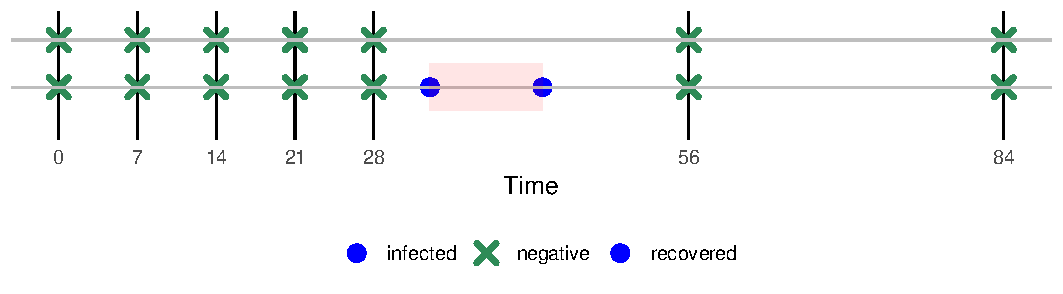
\includegraphics[width=1.2\textwidth]{cis-perfect-testing/truncation}}
  \caption[Undetected episodes in CIS data]{An unknown number of infection episodes in CIS are undetected. Consider the two individuals shown here: we collect identical data for them (a series of negative tests) yet the top individual was never infected and the bottom individual was. See the main text for why this is an issue. \label{perf-test:fig:truncation}}
\end{figure}

\subsection{Double interval censoring} \label{perf-test:sec:interval-censoring}

The second complication is that the infections are double interval censored.
The imprecision in the beginning of the infection episode arises because the only observation that episode $j$ has started is that an individual was negative at one test, on day $l_j^{(b)}-1$ (the minus one is because the first day that the infection could have begun is the day after the negative test), and positive at the next test, on day $r_j^{(b)}$.
Similarly, the end of the infection episode is bounded by the final positive test on day $l_j^{(e)}$ and the following negative test on day $r_j^{(e)}+1$ (the plus one is because the last day that the infection could have ended is the day before the negative test).
\Cref{perf-test:fig:double-interval-censor} shows this issue graphically.
\begin{figure}
  \centering 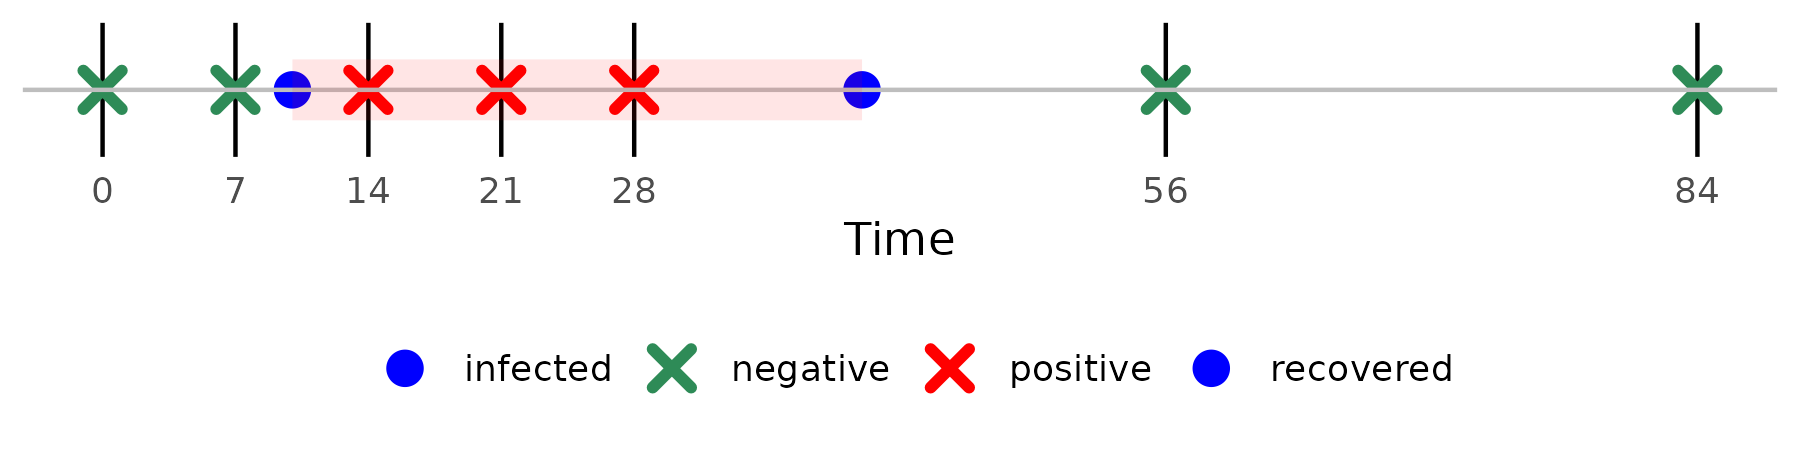
\includegraphics{cis-perfect-testing/double-interval-censor}
  \caption[Double-interval censoring in CIS data]{Episodes data in CIS is double interval censored, meaning that both the start and end of the episode are only known up to an interval. Demonstrated here by a participant who is recorded negative at time 7 to positive at time 14, bounding the start of the episode; similarly, changing from positive at time 28 to negative at time 56 bounds the end of the episode. \label{perf-test:fig:double-interval-censor}}
\end{figure}

\subsection{False negatives}

Write something about false negatives being common.

In this section, I introduce a probabilistic model for the generation of false negatives.
The simplest model for false negatives is a constant, non-zero probability of returning a negative test when detectable.
That is the test sensitivity, $\psens$, is less than 1.

A better model would be to allow the rate of false negatives to vary over the course of an episode.
False negatives are more likely to occur when the viral load of an individual is low, because there is less virus in their body to sample.
In \cref{E-ATACCC}, this mechanism is incorporated by viewing negative tests as a left-truncation of the observation noise (see \cref{E-ATACCC:sec:observation-modification}).
This observation suggests that a model with a declining test sensitivity as a function of time since infection might be more suitable.

The CIS data provides evidence for a test sensitivity declining over the course of an episode.
\Cref{imperf-test:fig:bounding-cis-sensitivity} demonstrates this by using the following classification for test results.
\begin{enumerate}
    \item All positive results are true positives.
    \item All intermittent negatives are false negatives.
    \item The negative at the end of an episode is a possible false negative.
    \item All other negatives are true negatives.
\end{enumerate}
Here, I am assuming that the probability of two false negative tests at the end of an episode is negligible.
As test sensitivity is the proportion of individuals who should test positive that do so, it can be empirically calculated as number of true positives / (number of true positives + number of false negatives).
Therefore, I calculate the test sensitivity for each day, considering the first positive result in an episode as day 0.
As the latent start day of the infection episode is before the first positive result, day 0 reflects some unknown number of days into the infection episode.
I bound the test sensitivity on each day by assuming either all or none of the possible false negatives (group 3) are in fact false negatives.
% In \cref{imperf-test:fig:bounding-cis-sensitivity} we consider the values produced by assuming the negative following the last positive in an episode could be either a true or false negative as a function of time since the individual was detected (\ie: the first positive test in the episode).
This generates broad bounds, although suggest a declining test sensitivity over the course of an episode (see \cref{imperf-test:fig:bounding-cis-sensitivity}).
Small numbers of tests mean that the series is noisy near the start and the end, such as both bounds being 0 on some days after day 40.
However, the general trend is clear.
\begin{figure}
  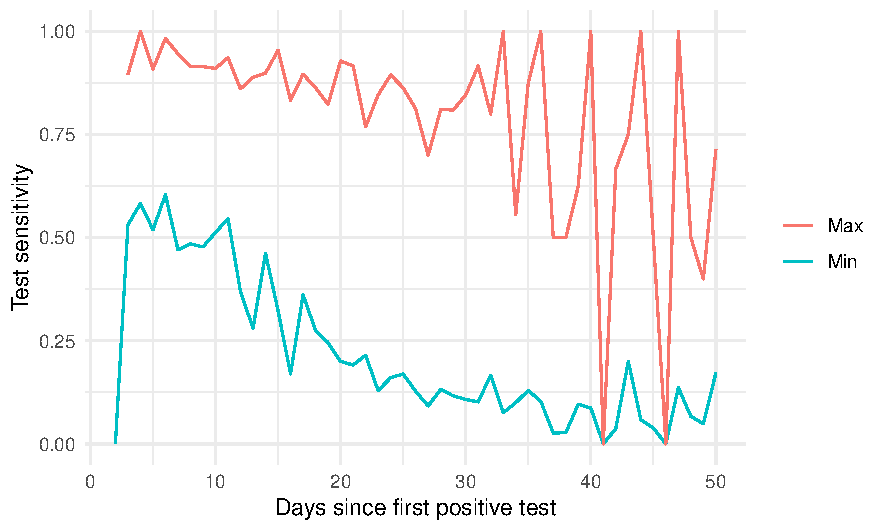
\includegraphics{cis-imperfect-testing/test-sens-bound}
  \caption[Bounding test sensitivity using CIS data]{
    Bounding the test sensitivity using CIS data as a function of time since the infection was detected.
  }
  \label{imperf-test:fig:bounding-cis-sensitivity}
\end{figure}

To assess the sensitivity of the procedure to a time-varying test sensitivity, it will be useful to simulate from a model with a varying test sensitivity as a function of days since the start of the infection episode.
Through consideration of \cref{imperf-test:fig:bounding-cis-sensitivity}, and the interaction of false negatives due to viral load in \cref{E-ATACCC}'s results, I propose the following model.
\begin{equation}
  p_\text{sens}(t) = \begin{cases}
    0.9 - \frac{0.9-0.5}{50}t &t \leq 50 \\
    0.5 &t > 50
  \end{cases}
  \label{imperf-test:eq:variable-test-sensitivity}
\end{equation}
where $t$ is the number of days since infection.
Therefore, this model consists of a linear decline in test sensitivity, before a constant minimum point.

Under this model, each test result in a detectable individual is an iid Bernoulli random variable with a probability $\psens$ of producing a positive.
As previously, tests in individuals without ongoing infection episodes are always negative.
I modified the simulation study from \cref{E-perf-test:sec:simulation-study} to generate test results in this way.

Following the modification, more single positive episodes are seen at lower values of $\psens$, with a value between 60\% and 80\% reproducing the number of single positive episodes observed in the CIS data (see \cref{imperf-test:fig:sim-single-pos}).
This is expected: a lower $\psens$ means that multiple positive tests are less likely, and hence the probability of a single positive episode is higher.

External information (see \cref{sec:ATACCC-analysis}) gives that $\psens$ is 95\% (95\% CrI: 93--96\%).
The requirement for a much lower value of $\psens$ in the simulation study here suggests this model of false negatives is inadequate.

\section{Related work}

Few studies look at the combination of both double interval censoring and undetected (or truncated) events.
This is especially true within the human biostatistical literature.
The literature does include theoretical frameworks which include the double censored and truncated case~\autocite{turnbullEmpirical,dempsterMaximum}, yet these frameworks have only been applied when the terminating event was either uncensored or right censored~\autocite{sunEmpirical,bacchettiNonparametric}.
These studies \autocite[and elsewhere, e.g.:][]{shenNonparametric} take a conditional likelihood approach.
They condition on the truncation (a selection effect) and the period where the initiating event occurs, which provides negligible information on the distribution of interest.
This is not the case for the CIS.
In CIS, infection episodes are more likely to be detected when an individual is in the weekly testing phase.
Therefore, the probability of an infection episode being detected conditional on being infected is higher than the overall probability of being detected.

Censored and truncated data are normal for estimation of the survival time of bird and insect nests~\autocite{heiseyABCs}.
\textcite{heiseyModelling} developed a framework for handling this situation.
The framework is general, allowing for arbitrary censoring patterns and double interval censoring.
They apply it to a situation the visit times are global (all nests could be detected on the same days), simplifying the likelihood.
I adapt this framework for CIS, when each individual has their own visit schedule (see section \cref{perf-test:sec:model}).
This framework is itself based long-standing methodology~\autocite{dempsterMaximum,turnbullEmpirical}.

The inclusion of false negatives into survival analysis is an area of much interest, especially in the application of tests for HIV in infants~\autocite[e.g.][]{brownBayesian,balasubramanianEstimation};
\textcite{piresIntervalMisclassify} provide a comprehensive review of approaches.
However, including false negatives with either doubly censored or truncated data has not been addressed.
The situation here requires both.

Similar likelihoods have previously appeared in the literature~\autocite[e.g.][eq.\ (2)]{piresIntervalMisclassify}.
However, this prior work was for singly interval censored data; incorporating the double interval censored nature of the CIS data will involve summing over the possible episode start times.


\section{Methodology}

\subsection{Survival analysis framework}

First, we consider the situtation without false negatives.
This approach extends the framework of \textcite{heiseyModelling} to include individuals without detected episodes.
I augment the data set with the full number of episodes, including those that are undetected.

Integrating over the number of missed episodes is possible analytically.
This makes inference tractable within modern, high-performance Bayesian software such as Stan.
Let the total number of infection episodes in the cohort be $\ntot = \ndet + \nnodet$ where $\ndet$ is the number of detected infections and $\nnodet$ is the number of undetected infections.
Let $\Ncis$ be the number of individuals in the cohort and $\nsched$ be the number of test schedules.
%Without loss of generality, let the individuals with a detected episode be indexed by $i = 1, \dots, \ndet$ and the individuals without a detected episode be indexed by $i = \ndet + 1, \dots, \Ncis$.
Let $i = 1, \dots, \nsched$ index infection schedules and $j = 1, \dots \ntot$ index infection episodes.

All the relevant information about episode $i$ can be fully characterised by the (unobserved) triplet $(b_j, e_j, \sched_j)$ where $b_j$ and $e_j$ are the times the episode being and end respectively and $\sched_j$ is the set of test times for the individual in which the episode occurs.
The episode's duration is $d_j = e_j - b_j + 1$.
%, the number of days the individual in which the episode occurred, was positive for 
This triplet is assumed iid.

$b_j$ and $e_j$ span possible infection and recovery times.
$\sched_j$ is one of the observed test schedules, with any other test schedule assumed to occur with probability zero.
Over the short period of time considered, each unique test schedule has zero or one detected episodes.

Let $i \in \set{D}$ indicate $\sched_i$ is associated with a detected episode.
That is, $i \in \set{D}$ if and only if there exists a $j(i)$ such that $b_{j(i)}$ and $e_{j(i)}$ such that $(b_{j(i)}, e_{j(i)}, \sched_i)$ is a detected episode.
$(b_{j(i)}, e_{j(i)}, \sched_i)$ is a detected episode when the following three conditions are met.
First, $\exists t \in \sched_i$ such that $b_{j(i)} \leq t \leq e_{j(i)}$; this condition is equivalent to having at least one positive test for the episode.
Second, $\exists t \in \sched_i$ such that $t < b_{j(i)}$, to lower bound the start of the episode.
Finally, $\exists t \in \sched_i$ such that $t > e_{j(i)}$, to upper bound the end of the episode; this condition will be met for any episode sufficiently far in the past in individuals not lost to follow-up (almost always the case in this context).
For a new context where recent infections need to be considered, this condition can be relaxed by considering these episodes as rightcensored, at little cost except a more complicated likelihood expression.


To relate the state space to the data, I define three subsets partitioning the space of possible infection and recovery times (\ie: are strict subsets of $T \times T$), for a test schedule $\sched_i$.
Figure \ref{perf-test:fig:partitionSpace} shows this graphically.
Each episode, whether detected or not, must fall into one of these three classes with a probability that is a function of the model parameters, $\theta$.

\begin{itemize}
\item
  Admissible episodes, $\alpha_i$, which have an infection and recovery time consistent with the data observed.
  This space is empty for $i \notin \set{D}$; in this case, $n_{ia} = 0$ admissible episodes occurred in individuals with test schedule $\sched_i$.
  Otherwise, $i \in \set{D}$ then $n_{ia} =1$ admissible episode occurred in an individual with test schedule $\sched_{i}$.
  Conditional on the episode occurring in individuals with test schedule $\sched_i$, it is admissible with probability $p_{ia} = \prob((b, e) \in \alpha_i \mid \theta)$.
  \label{perf-test:def:admissible}
\item
  Undetected episodes, $\Omega_i^C$, which have an infection and recovery time such that they would not have tested positive.
  An unknown number, $n_{iu}$ of these observed in individuals with test schedule $\sched_i$.
  Conditional on the episode occurring in individuals with test schedule $\sched_i$, it is undetected with probability $p_{iu} = \prob((b, e) \in \Omega^C_i \mid \theta)$.
\item
  Inadmissible episodes, $\beta_i$, which are not consistent with the data observed but would have been
  detected.
  This is all remaining episodes not in the previous sets.
  $n_{i\bar{a}} = 0$ of these occurred in any individuals with test schedule $\sched_i$.
  Conditional on the episode occurring in these individuals, it is inadmissible with probability $p_{i\bar{a}} = \prob((b, e) \in \beta_i \mid \theta)$.
\end{itemize}

% The detected region, $\Omega_i = \alpha_i \cup \beta_i$, for test schedule $\sched_i$ is the region where we could have observed episodes. 
% The notation is for consistency with \textcite{heiseyModelling}.
% $\Omega_i$ is the complement of $\Omega^C_i$.

\begin{figure}
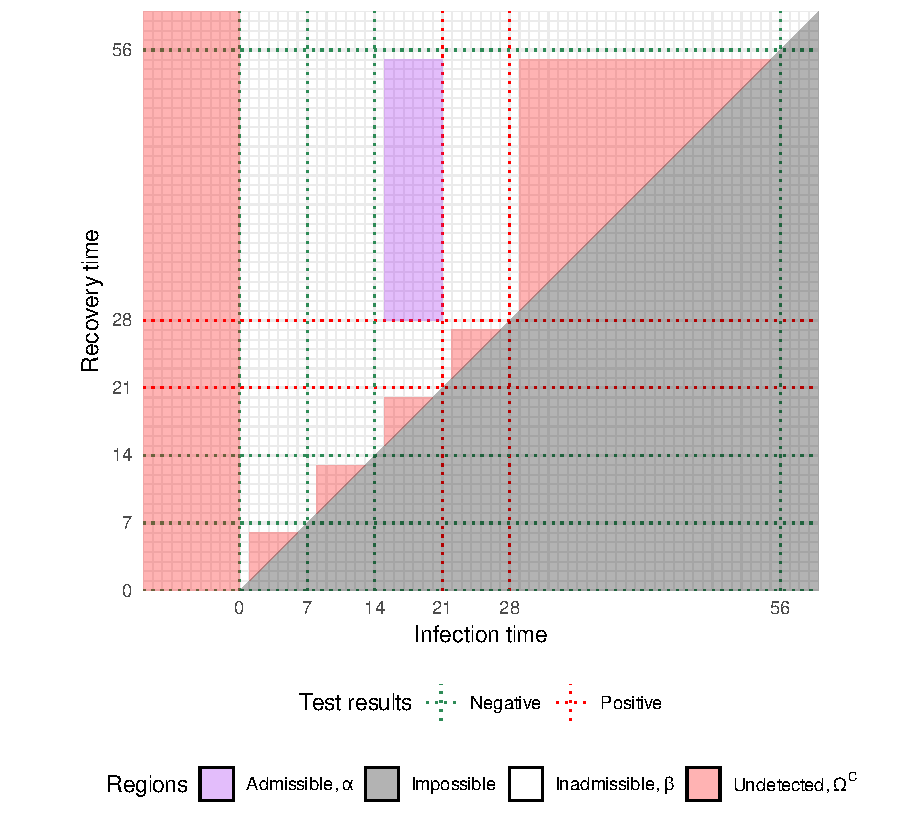
\includegraphics[width=\textwidth]{cis-perfect-testing/regions_diag}
\caption[Admissible, inadmissible, and undetected infections]{The regions (as defined in the main text) for an individual with test schedule $\sched_i$ whose first test was at time 0 and negative, with subsequent
negative tests at times 7, 14, and 56, and positive tests at times 21
and 28. Inadmissible region is unshaded. The black (impossible) region is because it does not make sense for recovery to occur prior to infection. \label{perf-test:fig:partitionSpace}}
\end{figure}

These three classes span all possible episodes and are mutually exclusive.
Hence, $\ntot = \ndet + \nnodet + n_{i\bar{a}} = \sum_{i=1}^{\nsched} n_{ia} + \sum_{i=1}^{\nsched} n_{iu} + 0$.
Furthermore, for all $i$, $p_{ia} + p_{iu} + p_{i\bar{a}} = 1$.

Any episode $j$ independently belongs to one of these classes.
I assume the individual in which each episode occurs is iid uniform across the cohort.
Therefore, conditional on $\ntot$, the number of episodes in each class, $(n_{ia}, n_{iu}, n_{i\bar{a}})^T$, are distributed multinomially.
The above probabilities ($p_{iu}$, $p_{ia}$, and $p_{i\bar{a}}$) are conditional on the episode occurring with test schedule $\sched_i$.
These probabilities are multiplied by $\eta_i/\Ncis$, where $\eta_i$ is the number of individuals with test schedule $\sched_i$, to give the probability that an episode belongs to each class, without conditioning on a specific individual.

The undetected classes for each individual cannot be distinguished by any observable data.
Each class's count needs to be marginalised over to calculate the likelihood.
Because the counts have a joint multinomial distribution, this is equivalent to only considering the sum of the counts.
The overall probability of an episode being unobserved is $\pnodet = \frac{1}{\Ncis} \sum_{i=1}^{\nsched} \eta_i p_{iu}$.
Furthermore, the inadmissible classes are guaranteed to have zero episodes.
Counts of zero do not contribute to a multinomial pmf (they multiply by 1).
Therefore, I combine the undetected classes into a single class and ignore the inadmissible classes.

Let $\na = (n_{1a}, \dots, n_{\nsched a})^T$ be the vector of counts of episodes in the admissible classes.
The counts $\na$ and $\nnodet$ are jointly distributed multinomially.
The support of the distribution requires $\nnodet = \ntot - \sum_{i=1}^{\nsched} n_{ia} = \ntot - \ndet$ and $\ntot \geq \ndet$.
Hence:
\begin{align}
p(\na \mid \ntot, \theta)
&= p(\nnodet, \na\mid \ntot, \theta) \\
&= \frac{\ntot!}{\nnodet! \prod_{i=1}^{\nsched} n_{ia}!}  \pnodet^{\nnodet}\prod_{i=1}^{\nsched} \left(\frac{1}{\nsched}p_{ia}\right)^{n_{ia}} \\
&\propto \frac{\ntot!}{(\ntot - \ndet)!} \pnodet^{\ntot - \ndet} \prod_{i \in \set{D}} p_{ia} \label{perf-test:eq:augmented-likelihood}
\end{align}
the final line follows because $\nnodet = \ntot - \ndet$, $n_{ia} = 1$ for $i \in \set{D}$, and $n_{ia} = 0$ otherwise.

In forming the probability $p_{ia}$, the data is used.
This is not quite correct because the cell probabilities in the likelihood should not depend on the data.
However, an alternative where each combination of infection and recovery times is considered its own class is possible.
Then, the counts for all the classes that previously contained undetected episodes would be zero.
The resulting likelihood would be the same.
Therefore, I present this version as it is clearer.

The posterior density we are interested in is $p(\theta \mid \na)$.
It can be written as follows.
\begin{align}
p(\theta \mid \na)
&\propto p(\theta) p(\na \mid \theta) \\
&= p(\theta) \sum_{\ntot=\ndet}^\infty p(\ntot \mid \theta) p(\na \mid \theta, \ntot) \\
&\propto p(\theta) \sum_{\ntot=\ndet}^\infty \left( p(\ntot \mid \theta) \frac{\ntot!}{(\ntot - \ndet)!} \pnodet^{\ntot - \ndet} \prod_{i \in \set{D}} p_{ia} \right) \\
&= p(\theta) \left( \prod_{i \in \set{D}} p_{ia} \right) \left( \sum_{\ntot=\ndet}^\infty p(\ntot \mid \theta) \frac{\ntot!}{(\ntot - \ndet)!} \pnodet^{\ntot - \ndet} \right) \label{perf-test:eq:full-posterior}.
\end{align}
The rest of this section derives expressions for each $p_{ia}$, $p_{u}$ and the sum.

To start, I derive an analytical solution to $\sum_{\ntot=\ndet}^\infty p(\ntot \mid \theta) \frac{\ntot!}{(\ntot - \ndet)!} \pnodet^{\ntot - \ndet}$ under the prior $\ntot \dist \NBc(\mu, r)$.
I assume that $\theta$, which are only the parameters of the survival distribution, has a prior independent of $\ntot$, the number of infections that occurred in the cohort.
Therefore, $p(\ntot \mid \theta) = p(\ntot)$.
Putting a negative binomial prior on $\ntot$ is equivalent to the following gamma-Poisson composite; its use simplifies the derivation.
\begin{align}
\ntot \mid \lambda &\dist \Poi(\lambda) \\
\lambda &\dist \GamDist(a, b)
\end{align}
where $b = r / \mu$ and $a = r$.
Hence:
\begin{align}
&\sum_{\ntot=\ndet}^\infty \frac{\ntot!}{(\ntot-\ndet)!} \pnodet^{\ntot-\ndet} p(\ntot) \\
&= \int \sum_{\ntot=\ndet}^\infty \frac{\ntot!}{(\ntot-\ndet)!} \pnodet^{\ntot-\ndet} p(\ntot \mid \lambda) p(\lambda) d\lambda &\text{$\lambda$ explicit}\\
&= \int \sum_{\ntot=\ndet}^\infty \frac{\ntot!}{(\ntot-\ndet)!} \pnodet^{\ntot-\ndet} \frac{\lambda^{\ntot} e^{-\lambda}}{\ntot!} p(\lambda) d\lambda &\ntot \dist \Poi\\
%&= \int \sum_{\ntot=\ndet}^\infty \frac{1}{(\ntot-\ndet)!} \pnodet^{\ntot-\ndet} \lambda^{\ntot-\ndet} \lambda^{\ndet} e^{-\lambda} p(\lambda) d\lambda \\
&= \int \lambda^{\ndet} e^{-\lambda} p(\lambda) \sum_{\nnodet=0}^\infty \frac{(\pnodet \lambda)^{\nnodet}}{\nnodet!} d\lambda &\nnodet = \ntot-\ndet\\
&= \int \lambda^{\ndet} e^{-\lambda} p(\lambda) e^{\lambda \pnodet} d\lambda &\text{Maclaurin series of $e$} \\
&= \int \lambda^{\ndet} e^{-\lambda(1 - \pnodet)} \frac{b^a}{\Gamma(a)} \lambda^{a-1} e^{-b\lambda} \lambda d\lambda &\text{Gamma pdf}\\
&= \int \frac{b^a}{\Gamma(a)} \lambda^{a+\ndet-1} e^{-(b+1-\pnodet)\lambda} \lambda d\lambda \\
&= \frac{b^a}{\Gamma(a)} \frac{\Gamma(a+\ndet)}{(b+1-\pnodet)^{a+\ndet}} &\text{Gamma pdf}\\
&\propto (b+1-\pnodet)^{-(a+\ndet)} \\
&= (r/\mu + 1 - \pnodet)^{-(r+\ndet)} &\text{sub in $\mu$ and $r$}\\
&\propto(r + \mu (1- \pnodet))^{-(r+\ndet)}.
\end{align}

Substituting this into \cref{perf-test:eq:full-posterior} gives:
\begin{align}
p(\theta \mid \na)
&\propto p(\theta) \left( \prod_{i \in \set{D}} p_{ia} \right) (r + \mu (1- \pnodet))^{-(r+\ndet)} \label{perf-test:eq:full-posterior-simplified}.
\end{align}

Next, I derive $p_{ia}$.
By definition (see~\cpageref{perf-test:def:admissible}), we have, for any $i \in \set{D}$:
\begin{align}
p_{ia} &= \prob((b, e) \in \alpha_i \mid \theta) \\
\alpha_i &= \{ (b, e) : l_{j(i)}^{(b)} \leq b \leq r_{j(i)}^{(b)} \wedge l_{j(i)}^{(e)} \leq e \leq r_{j(i)}^{(e)}\}.
\intertext{Suppressing the conditioning on $\theta$, this gives:}
p_{ia}
&= \prob \left( l_{j(i)}^{(b)} \leq B_{j(i)} \leq r_{j(i)}^{(b)}, l_{j(i)}^{(e)} \leq E_{j(i)} \leq r_{j(i)}^{(e)} \right) \\
&= \prob \left( l_{j(i)}^{(e)} \leq E_{j(i)} \leq r_{j(i)}^{(e)} \mid l_{j(i)}^{(b)} \leq B_{j(i)} \leq r_{j(i)}^{(b)} \right) \prob \left( l_{j(i)}^{(b)} \leq B_{j(i)} \leq r_{j(i)}^{(b)} \right) \\
&=\sum_{b = l_{j(i)}^{(l)}}^{r_{j(i)}^{(b)}} \prob \left( l_{j(i)}^{(e)} \leq E_{j(i)} \leq r_{j(i)}^{(e)} \mid B_{j(i)} = b \right) \prob \left(B_{j(i)} = b \right) \\
&=\sum_{b = l_{j(i)}^{(b)}}^{r_{j(i)}^{(b)}} \prob \left( l_{j(i)}^{(e)} - b + 1 \leq D_{j(i)} \leq r_{j(i)}^{(e)} - b + 1 \right) \prob \left(B_{j(i)} = b \right) &\text{by def of $D_{j(i)}$} \\
&=\sum_{b = l_{j(i)}^{(b)}}^{r_{j(i)}^{(b)}} \left( S_\theta(l_{j(i)}^{(e)} - b + 1) - S_\theta(r_{j(i)}^{(e)} - b + 1) \right) \prob \left(B_{j(i)} = b \right) &\text{by def of $S_\theta$} \\
&\propto \sum_{b = l_{j(i)}^{(b)}}^{r_{j(i)}^{(b)}} \left( S_\theta(l_{j(i)}^{(e)} - b + 1) - S_\theta(r_{j(i)}^{(e)} - b + 1) \right)
\end{align}
under the assumption of uniform probability of infection time.

The next step is to derive $1 - p_u = 1 - \frac{1}{N} \sum_{i=1}^{\nsched} p_{iu} = \frac{1}{N} \sum_{i=1}^{\nsched} (1 - p_{iu})$.
Therefore, the crucial component is $1 - p_{iu} = 1 - \prob((B_{j(i)}, E_{j(i)}) \in \Omega^C_i \mid \theta)$, one minus the probability that episode $i$ was undetected.
An episode is undetected if and only if no tests are performed during the episode or if there was no negative test prior to the episode.
Equivalently, that the first test at or after $b$ is after $e$, or that there is no negative test prior to $b$.
To formalise this, first define $\tau_{\sched_i}(t)$ as the time until the next test at or after time $t$ in the schedule $\sched_i$:
\begin{align}
\tau_{\sched_i}(t) &= \min \{ t' \in \sched_i : t' \geq t \} - t.
\end{align}
Then $\Omega^C_i$ can be written as:
\begin{align}
\Omega_i^C = \{ (b, e) \ssep \tau_{\sched_i}(b) + b > e \vee b \leq \min(\sched_i) \}.
\end{align}
Therefore, suppressing the conditioning on $\theta$:
\begin{align}
1 - p_{iu}
&= 1 - \prob((B_{j(i)}, E_{j(i)}) \in \Omega^C_i) \\
&= 1 - \prob( \tau_{\sched_i}(B_{j(i)}) + B_{j(i)} > E_{j(i)} \vee B_{j(i)} \leq \min(\sched_i) ) \\
&= 1 - \prob( \tau_{\sched_i}(B_{j(i)}) + 1 > D_i , B_{j(i)} > \min(\sched_i) )  - \prob( B_{j(i)} \leq \min(\sched_i) ) \\
&= 1 - \sum_{b={\min\sched_i} + 1}^T \prob( \tau_{\sched_i}(b) + 1> D_i) \prob(B_{j(i)} = b) - \sum_{t=1}^{\min\sched_i} \prob(B_{j(i)} = b)\\
&= 1 - \frac{1}{T} \sum_{b=\min(\sched_i)+1}^T (1 - S_\theta(\tau_{\sched_i}(b) + 1)) - \frac{1}{T} \min\sched_i \\
&= \frac{1}{T} \left(T - \sum_{b=\min\sched_i+1}^T (1 - S_\theta(\tau_{\sched_i}(b) + 1)) - \min\sched_i \right) \\
&= \frac{1}{T} \left(T - (T - \min\sched_i) + \sum_{b=\min\sched_i+1}^T S_\theta(\tau_{\sched_i}(b + 1)) - \min\sched_i \right) \\
&= \frac{1}{T} \sum_{b=\min(\sched_i)+1}^T S_\theta(\tau_{\sched_i}(b) + 1). \label{perf-test:eq:piu}
\end{align}

\subsection{False negatives}

Now we modify the survival framework to incorporate false negatives.
We use the model with a constant test sensitivity to ensure the likelihood remains tractable.

\subsubsection{Modifying \texorpdfstring{$p_{ia}$}{pia}} \label{imperf-test:sec:modifying-p_ia}

I will modify $p_{ia}$ to allow the negative test following the last positive to be a false negative.
If it is a false negative, then I will consider the episode's end right-censored.
However, if it is a true negative, then the episode's end is interval censored, as previously.
A mixture of these scenarios forms the episode's likelihood contribution, with the mixture probability determined by the test sensitivity.

I start by finding the tests that need consideration.
For tractability and simplicity, I consider only tests between the negative tests providing an upper bound on the length of the episode.
By definition (see \cref{E-biology-data:sec:cis-episodes}), these are the tests between $l_{j(i)}^{(b)} - 1$ and $r_{j(i)}^{(e)} + 1$ inclusive.
They are a subset of $\sched_i$, the set of test times for the individual in which episode $i$ occurs.

For tractability, assume that the negative test bounding the start of the episode, on day $l_{j(i)}^{(b)}-1$, is a true negative.
This assumption is reasonable because, since a positive test follows at $r_{j(i)}^{(b)}$, the negative at $l_{j(i)}^{(b)}-1$ is likely early in the infection and the test sensitivity is high early in an infection.
Therefore, this is unlikely to be a false negative because, if the individual was detectable at this time, they are in a period with high test sensitivity.
This true negative, occurs with probability 1, and hence does not contribute to the likelihood.
Denote the remaining tests considered as $\sched'_i = \{ t \in \sched_i \ssep r_{j(i)}^{(b)} \leq t \leq r_{j(i)}^{(e)} + 1 \}$, and their results by $\vec{y_{j(i)}} = \{ y_{j(i)}(t) \ssep t \in \sched'_i \}$ where $y_{j(i)}(t) = 1$ if the test on day $t$ is positive and 0 otherwise.

As I assume that there are no false positives, the infection episode must span at least the period $[r^{(b)}_{j(i)}, l^{(e)}_{j(i)}]$ because it starts and ends with a positive test.
This includes all $t \in \sched'_i$ except $t = r_{j(i)}^{(e)}+1$.
Therefore, the test results at times in $\sched_i'$, except the test at $r_{j(i)}^{(e)}+1$, are either true positives or false negatives.

Consider the negative test at $r_{j(i)}^{(e)}+1$, the first negative after the start of the episode which may be a false negative.
It is a false negative if and only if the episode ends after the test, \ie $e_{j(i)} > r_{j(i)}^{(e)}$.
I proceed by considering whether this is the case, and considering the case with $b_{j(i)}$ known; $b_{j(i)}$ will later be integrated out.

First, if $e_{j(i)} \leq r_{j(i)}^{(e)}$, meaning that the test at $r_{j(i)}^{(e)}+1$ is a true negative and the end of the episode is interval censored as in the previous chapter.
% In this case, the test at $r_{j(i)}^{(e)} + 1$ is a true negative, as are all other tests not in $\sched'_i$.
The true negative occurs with probability 1, by the assumption of no false positives.
\begin{align}
&p(\vec{y_{j(i)}}, e_{j(i)} \leq r_{j(i)}^{(e)} | b_{j(i)}, p_\text{sens}, \theta) \\
&= p(\vec{y_{j(i)}}, l_{j(i)}^{(e)} \leq e_{j(i)} \leq r_{j(i)}^{(e)} | t_i, b_{j(i)}, p_\text{sens}, \theta) \\ % &\text{as no false positives}
&= p(\vec{y_{j(i)}} \mid l_{j(i)}^{(e)} \leq e_{j(i)} \leq r_{j(i)}^{(e)}, t_i, b_{j(i)}, p_\text{sens}, \theta) p(l_{j(i)}^{(e)} \leq e_{j(i)} \leq r_{j(i)}^{(e)} | t_i, b_{j(i)}, p_\text{sens}, \theta) \\
&= \left( \prod_{t \in \sched'_i} p_\text{sens}^{y_{j(i)}(t)} (1 - p_\text{sens})^{(1 - y_{j(i)}(t))} \right) \left( S_\theta(l_{j(i)}^{(e)} - b_{j(i)} - 1) - S_\theta(r_{j(i)}^{(e)} - b_{j(i)} - 1) \right)
\label{imperf-test:eq:ll-ei-lt-ri}
\end{align}

Second, if $e_{j(i)} > r_{j(i)}^{(e)}$.
In this case, the test at $r_{j(i)}^{(e)}$ is a false negative, occurring with probability $(1 - p_\text{sens})$.
To avoid having to consider tests after $r_{j(i)}^{(e)}$, which could greatly complicate the likelihood, I model this case as the episode being right-censored at $r_{j(i)}^{(e)}$.
Taking the same approach as before:
\begin{align}
&p(\vec{y_{j(i)}}, e_{j(i)} > r_{j(i)}^{(e)} | b_{j(i)}, p_\text{sens}, \theta) \\
&= p(\vec{y_{j(i)}} \mid e_{j(i)} > r_{j(i)}^{(e)}, t_i, b_{j(i)}, p_\text{sens}, \theta) p(e_{j(i)} > r_{j(i)}^{(e)} | t_i, b_{j(i)}, p_\text{sens}, \theta) \\
&= \left( \prod_{t \in \sched'_i} p_\text{sens}^{y_{j(i)}(t)} (1 - p_\text{sens})^{(1 - y_{j(i)}(t))} \right) (1 - p_\text{sens}) S_\theta(r_{j(i)}^{(e)} - b_{j(i)} - 1)
\label{imperf-test:eq:ll-ei-gt-ri}
\end{align}

These expressions can now be used to form the full replacement for $p_{ia}$, $p'_{ia}$, the likelihood of the data $\vec{y_{j(i)}}$.
First, augment the data with $b_{j(i)}$, and split into the cases just discussed:
\begin{align}
p_{ia}'
&= p(\vec{y_{j(i)}} \mid p_\text{sens}, \theta) \\
&= \sum_{b_{j(i)} = l_{j(i)}^{(b)}}^{r_{j(i)}^{(b)}} \left( p(\vec{y_{j(i)}}, e_{j(i)} \leq r_{j(i)}^{(e)} \mid b_{j(i)}, p_\text{sens}, \theta) + p(\vec{y_{j(i)}}, e_{j(i)} > r_{j(i)}^{(e)} \mid b_{j(i)}, p_\text{sens}, \theta) \right) p(b_{j(i)} \mid p_\text{sens}, \theta).
\intertext{Now, substitute in \cref{imperf-test:eq:ll-ei-lt-ri,imperf-test:eq:ll-ei-gt-ri}, then take out the common factor:}
&= \left( \prod_{t \in \sched'_i} p_\text{sens}^{y_{j(i)}(t)} (1 - p_\text{sens})^{(1 - y_{j(i)}(t))} \right) \\ & \ \times \sum_{b_{j(i)} = l_{j(i)}^{(b)}}^{r_{j(i)}^{(b)}} \left( S_\theta(l_{j(i)}^{(e)} - b_{j(i)} - 1) - S_\theta(r_{j(i)}^{(e)} - b_{j(i)} - 1) + (1 - p_\text{sens}) S_\theta(r_{j(i)}^{(e)} - b_{j(i)} - 1) \right) \\ & \ \times p(b_{j(i)} \mid p_\text{sens}, \theta) \\
&= \left( \prod_{t \in \sched'_i} p_\text{sens}^{y_{j(i)}(t)} (1 - p_\text{sens})^{(1 - y_{j(i)}(t))} \right) \\ & \ \times \sum_{b_{j(i)} = l_{j(i)}^{(b)}}^{r_{j(i)}^{(b)}} \left( S_\theta(l_{j(i)}^{(e)} - b_{j(i)} - 1) - p_\text{sens} S_\theta(r_{j(i)}^{(e)} - b_{j(i)} - 1) \right) p(b_{j(i)} \mid p_\text{sens}, \theta).
\label{imperf-test:eq:pia-prime}
\end{align}
Note that if $p_\text{sens} = 1$ then $p_{ia}' = p_{ia}$.

If $\psens$ is fixed (\ie has a point prior) and $p(b_{j(i)} \mid \psens, \theta) \propto 1$ (as assumed in \cref{E-perf-test}) then:
\begin{align}
p_{ia}'
&\propto \sum_{b_{j(i)} = l_{j(i)}^{(b)}}^{r_{j(i)}^{(b)}} S_\theta(l_{j(i)}^{(e)} - b_{j(i)} - 1) - p_\text{sens} S_\theta(r_{j(i)}^{(e)} - b_{j(i)} - 1).
\label{imperf-test:eq:pia-prime-constant}
\end{align}

\subsubsection{Modifying \texorpdfstring{$p_{iu}$}{piu}} \label{imperf-test:sec:modifying-p_iu}

Several mechanisms for episodes being undetected were considered when deriving $p_{iu}$ in \cref{perf-test:eq:piu}.
I now consider the additional mechanisms arising due to false negatives.
Specifically, episode $i$ could be undetected if the first test after the $b_{j(i)}$, episode $i$'s start day, is a false negative and then there are no subsequent positive tests.

This false negative would occur at the first test after the infection episode begins, on day $b_{j(i)} + \tau_{\sched_i}(b_{j(i)})$ (see \cref{E-perf-test:sec:model}).
A false negative occurring requires that the episode has not yet ended but a negative still occurs.
The episode has not yet ended at the time of the test if $e_{j(i)} = b_{j(i)} + d_i - 1$ is after the test, that is the duration of the infection $d_i > \tau_{\sched_i}(b_{j(i)})$.
Conditional on the episode having not yet ended, the test result is negative with probability $1 - \psens$.

For there to be no subsequent positive tests, all tests up until day $e_{j(i)}$ are false negatives.
I assume there is a negligible probability of two false negatives.
Therefore, this can only occur if the episode ends before another test.
Denote the number of days between $b_{j(i)}$ and the test following the false negative as $\tau^2_{\sched_i}(b_{j(i)}) \stackrel{\text{def}}{=} \tau_{\sched_i}(\tau_{\sched_i}(b_{j(i)}) + 1)$.
Then, the episode ends before this test if $d_i < \tau^2_{\sched_i}(b_{j(i)})$.

Therefore, this mechanism causes episode $i$ to be undetected if all the following conditions hold.
\begin{enumerate}
    \item The episode would have been detected considering only the mechanisms in \cref{perf-test:eq:piu}. That is $b_{j(i)} > \min(\sched_i)$ and $\tau_{\sched_i}(b_{j(i)}) + b_{j(i)} \leq e_{j(i)}$.
    \item The episode ends in the interval $[\tau_{\sched_i}(b_{j(i)}) + b_{j(i)}, \tau^2_{\sched_i}(b_{j(i)}) + b_{j(i)}]$.
      Note that the lower bound here is exactly the bound on $e_{j(i)}$ in the previous condition.
      Equivalently, $\tau_{\sched_i}(b_{j(i)}) + 1 \leq d_i \leq \tau^2_{\sched_i}(b_{j(i)}) + 1$.
    \item A false negative occurs on day $\tau_{\sched_i}(b_{j(i)}) + b_{j(i)}$. Conditional on the previous condition, this occurs with probability $1 - \psens$.
\end{enumerate}

The probability of this occurring, conditional on $B_{j(i)} = b_{j(i)} > \min(\sched_i)$ is:
\begin{align}
&\prob \left(
    \tau_{\sched_i}(b_{j(i)}) + 1 \leq D_i \leq \tau^2_{\sched_i}(b_{j(i)}) + 1
    \mid b_{j(i)},
\theta \right) (1 - \psens) \\
&= \left( S_\theta(\tau_{\sched_i}(b_{j(i)}) + 1) - S_\theta(\tau^2_{\sched_i}(b_{j(i)}) + 1) \right) (1 - \psens).
\end{align}
Integrating over $b_{j(i)}$ for $\min \sched_i < b_{j(i)} \leq T$ ($T$ being the last day of the period considered), in the same way as \cref{perf-test:eq:piu}, gives:
\begin{align}
\eta = (1 - p_\text{sens})\frac{1}{T} \sum_{b=\min(\sched_i) + 1}^T \left( S_\theta(\tau_{\sched_i}(b) + 1) - S_\theta(\tau^2_{\sched_i}(b) + 1) \right).
\end{align}

Denote the replacement for $p_{iu}$ as $p_{iu}'$.
$p_{iu}'$ is the probability of episode $i$ being missed, considering both the mechanisms from \cref{E-perf-test} and the new mechanism here.
These mechanisms are mutually exclusive.
Hence, $p_{iu}'$ is the sum of these, $p_{iu}' = p_{iu} + \eta$.
For the posterior density, \cref{E-perf-test:eq:full-posterior}, $1 - p_{iu}'$ is the required quantity.
\begin{align}
1 - p_{iu}'
&= 1 - p_{iu} - (1 - p_\text{sens})\frac{1}{T} \sum_{b=\min(\sched_i) + 1}^T \left( S_\theta(\tau_{\sched_i}(b) + 1) - S_\theta(\tau^2_{\sched_i}(b) + 1) \right) \\
&= \frac{1}{T} \sum_{b=\min(\sched_i) + 1}^T \left( p_\text{sens} S_\theta(\tau_{\sched_i}(b) + 1) + (1 - p_\text{sens}) S_\theta(\tau^2_{\sched_i}(b) + 1)\right).
\label{imperf-test:eq:pit-prime}
\end{align}

$p_{iu}'$ and $p_{ia}'$ are substituted for $p_{iu}$ and $p_{ia}$ respectively in \cref{E-perf-test:eq:full-posterior}.
The posterior density is otherwise unchanged.



\subsection{Incorporating prior information}

\todo[inline]{A bunch of this can probably be cut / moved to supp material. Supp material should also contain the ATACCC analysis.}

The information from \cref{E-ATACCC} can be incorporated through the prior.
This is desirable because the ATACCC study frequently sampled individuals early in the infection.
Therefore, \cref{E-ATACCC}'s estimate of the survival distribution in the early infection period should be reliable.
In the later infection period, the ATACCC study has fewer observations and hence the estimates are less reliable.
CIS can inform the posterior in this region.

When constructing the prior, two aspects need consideration.
Firstly, the model structure from \cref{E-ATACCC} leads to positive correlation in the posterior estimates of the hazard, which should be propagated into this analysis.
That is, the prior used in this analysis cannot be independent across the hazards.
Secondly, the uncertainty in the estimates from \cref{E-ATACCC} should be increased for this analysis.
The additional uncertainty is because the \cref{E-ATACCC} analysis extrapolates beyond the data using strong model assumptions (see \cref{E-ATACCC:sec:discussion}).
%Furthermore, there are differences in the study design and laboratories used between the two studies (see \cref{E-intro:sec:studies}) which may mean that results do not generalise between the studies.
I form the prior for the combination in two steps.

I first approximate the \cref{E-ATACCC} posterior estimate of the hazard as a multivariate normal on the logit scale.
This can be viewed as an approximation of Markov melding~\autocite{goudieJoining}.
Using a multivariate normal, as opposed to multiple univariate distribution, ensures that the correlation between the hazards is preserved.
The logit transformation maps from the $[0, 1]$ interval to the full real line.
To estimate the parameters of the multivariate normal, I use the method of moments.
The approximation is very good (see \cref{perf-test:fig:approximate-ATACCC-hazard} and \cref{perf-test:fig:approximate-ATACCC-survival}).
\begin{figure}
  \thisfloatpagestyle{empty}
  \vspace{-2.5cm}
  \makebox[\textwidth][c]{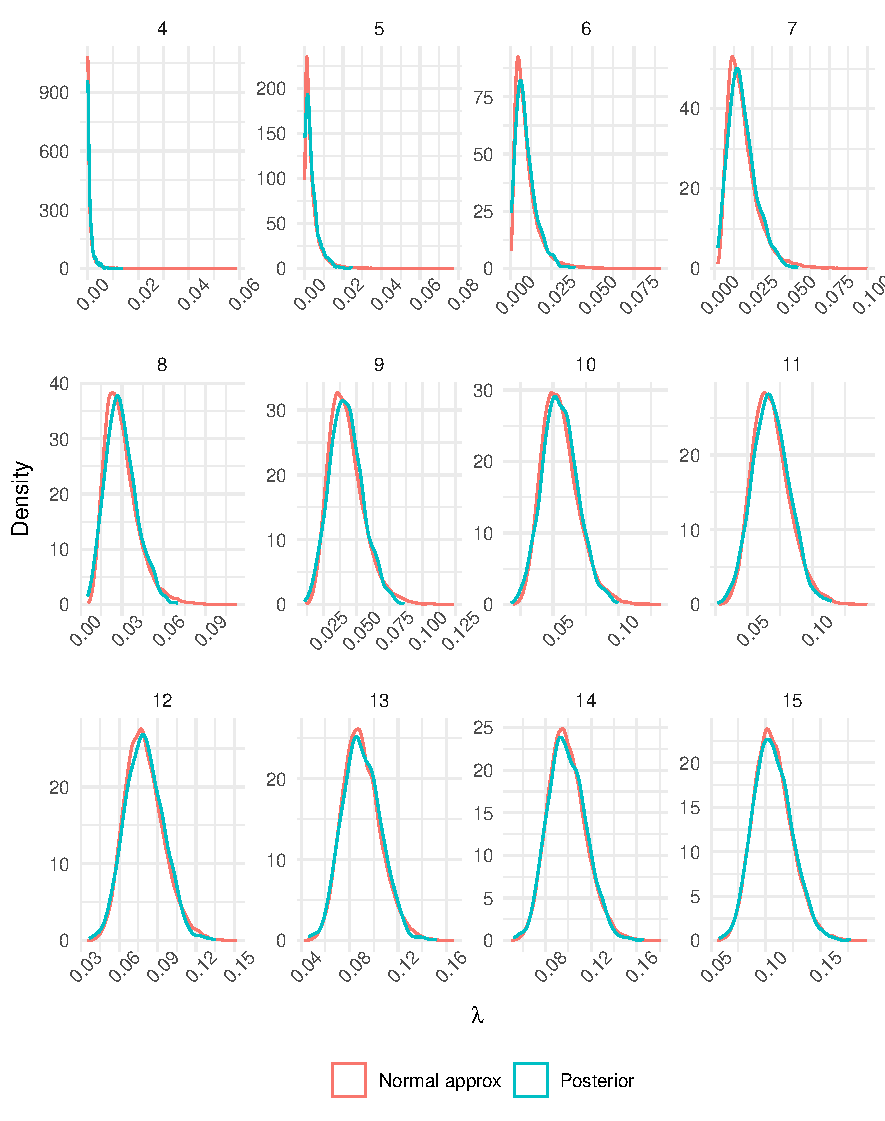
\includegraphics[width=.9\paperwidth]{cis-perfect-testing/ataccc-approximation-hazard}}
  \caption[Approximating the ATACCC posterior hazard as a logit-normal]{Comparison of the posterior estimate of the hazard from \cref{E-ATACCC} and its approximation with a logit-normal distribution (kernel density estimate smoothed) for the first 15 hazards. \label{perf-test:fig:approximate-ATACCC-hazard}}
\end{figure}
\begin{figure}
  \centering 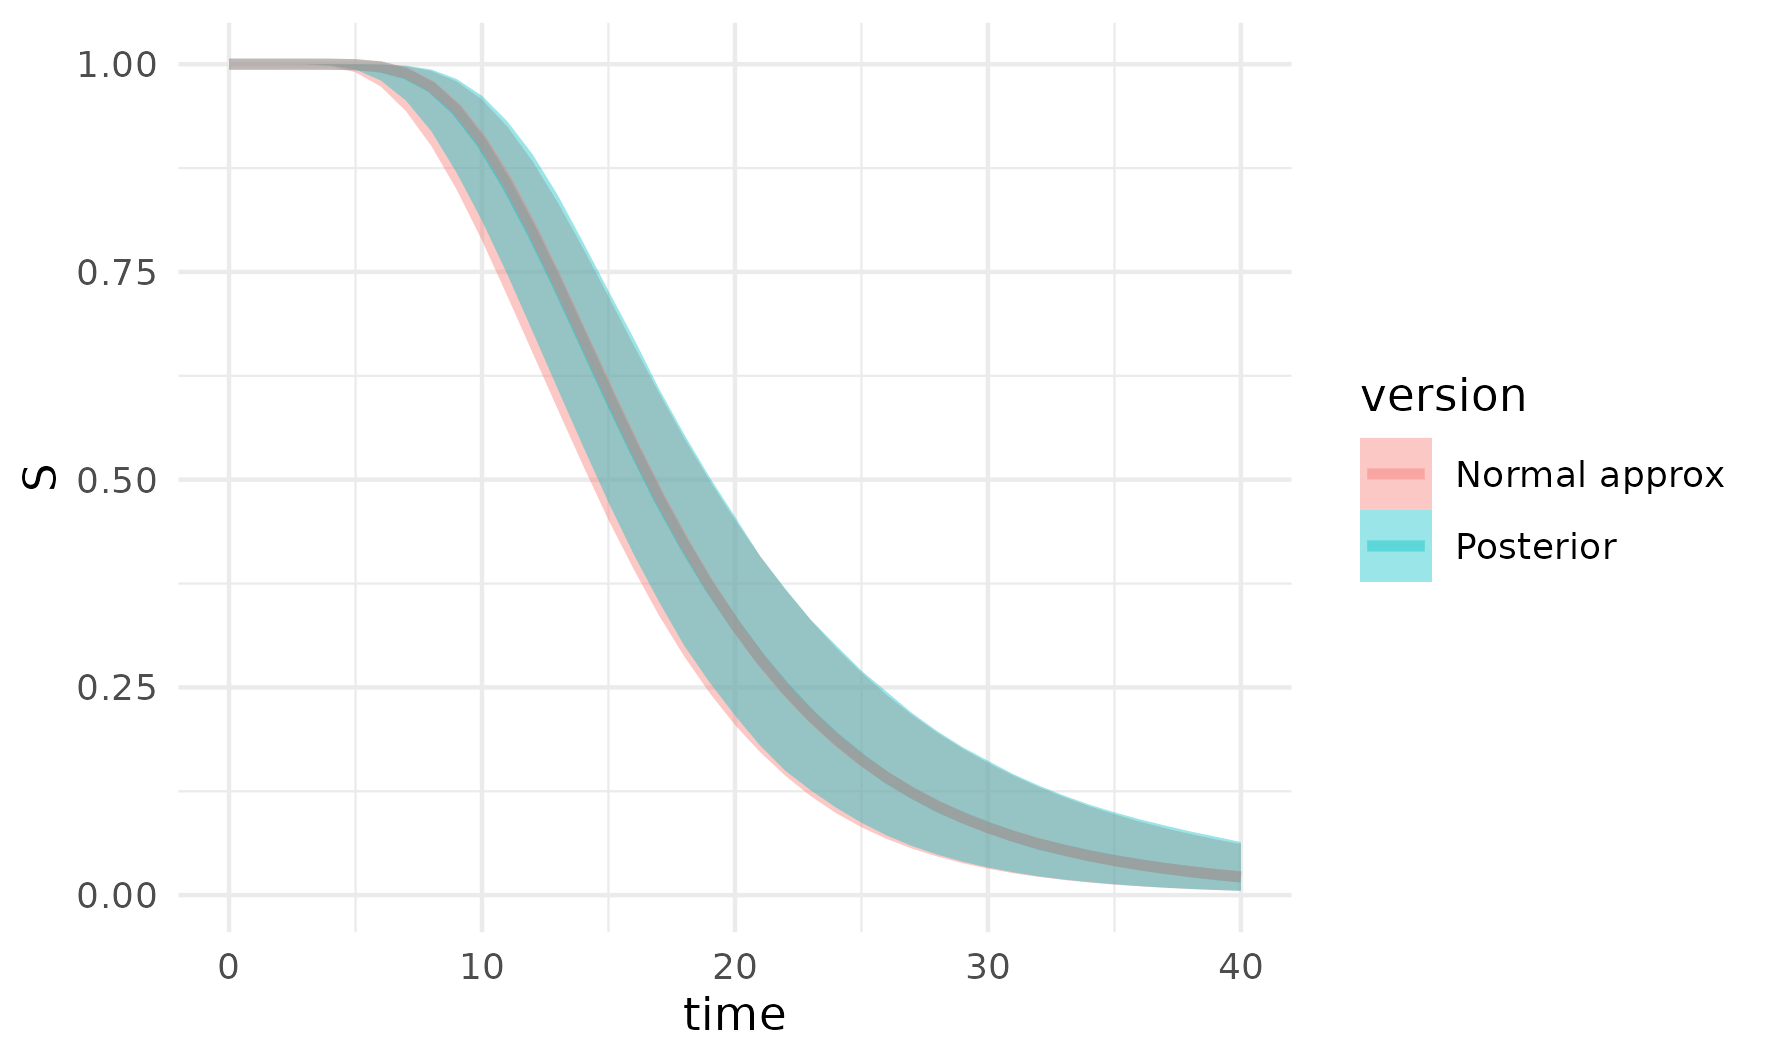
\includegraphics{cis-perfect-testing/ataccc-approximation-survival}
  \caption[Approximating the ATACCC posterior survival as a logit-normal]{Comparison of the posterior estimate of the survival from \cref{E-ATACCC} and its approximation with a logit-normal distribution (median and central 95\% interval). The survival is a function of all the hazards up until that point, therefore the correlation between the hazards must be well-approximated to have these agree. \label{perf-test:fig:approximate-ATACCC-survival}}
\end{figure}

Having approximated the estimate as a multivariate normal, I add additional uncertainty using a discrete Beta process.
The discrete Beta process prior generalises the form of prior used in \cref{perf-test:sec:independent-priors} by allowing the central estimate of the hazard to vary over time~\autocite{ibrahimBayesian,sunStatisticala}.
It is:
\begin{align}
  \lambda_t &\sim \text{Beta}(\alpha_t, \beta_t) &t = 1, 2, \dots \\
  \alpha_t &= k_t h_t + \alpha_0 \\
  \beta_t &= k_t (1 - h_t) + \beta_0
\end{align}
where $k_t$, $\alpha_0$, and $\beta_0$ are hyperparameters; and $h_t$ is a point estimate of the hazard at time $t$ from ATACCC.
An intuition for what this distribution represents can be gained from a conjugate model for $\lambda_t$ with a beta prior and a binomial likelihood.
If $\lambda_t$ is given the prior distribution $\text{Beta}(\alpha_0, \beta_0)$, and we then have $k_t$ observations with $k_t h_t$ successes, then the posterior distribution for $\lambda_t$ is $\text{Beta}(\alpha_t, \beta_t)$ (as defined above).

$k_t$ reflects the subjective belief that the estimates from \cref{E-ATACCC} are very reliable in the early infection period but unreliable by day 30.
The equation for $k_t$ is below and shown in \cref{perf-test:fig:kt}.
\begin{align}
k_t = \begin{cases}
  \expit(-0.4 * (t - 20)) &\text{for $t \leq 39$} \\
  0 &t > 39
\end{cases}
\end{align}
where $\expit(x) = 1 / (1 + \exp(-x))$.

\begin{figure}
  \centering 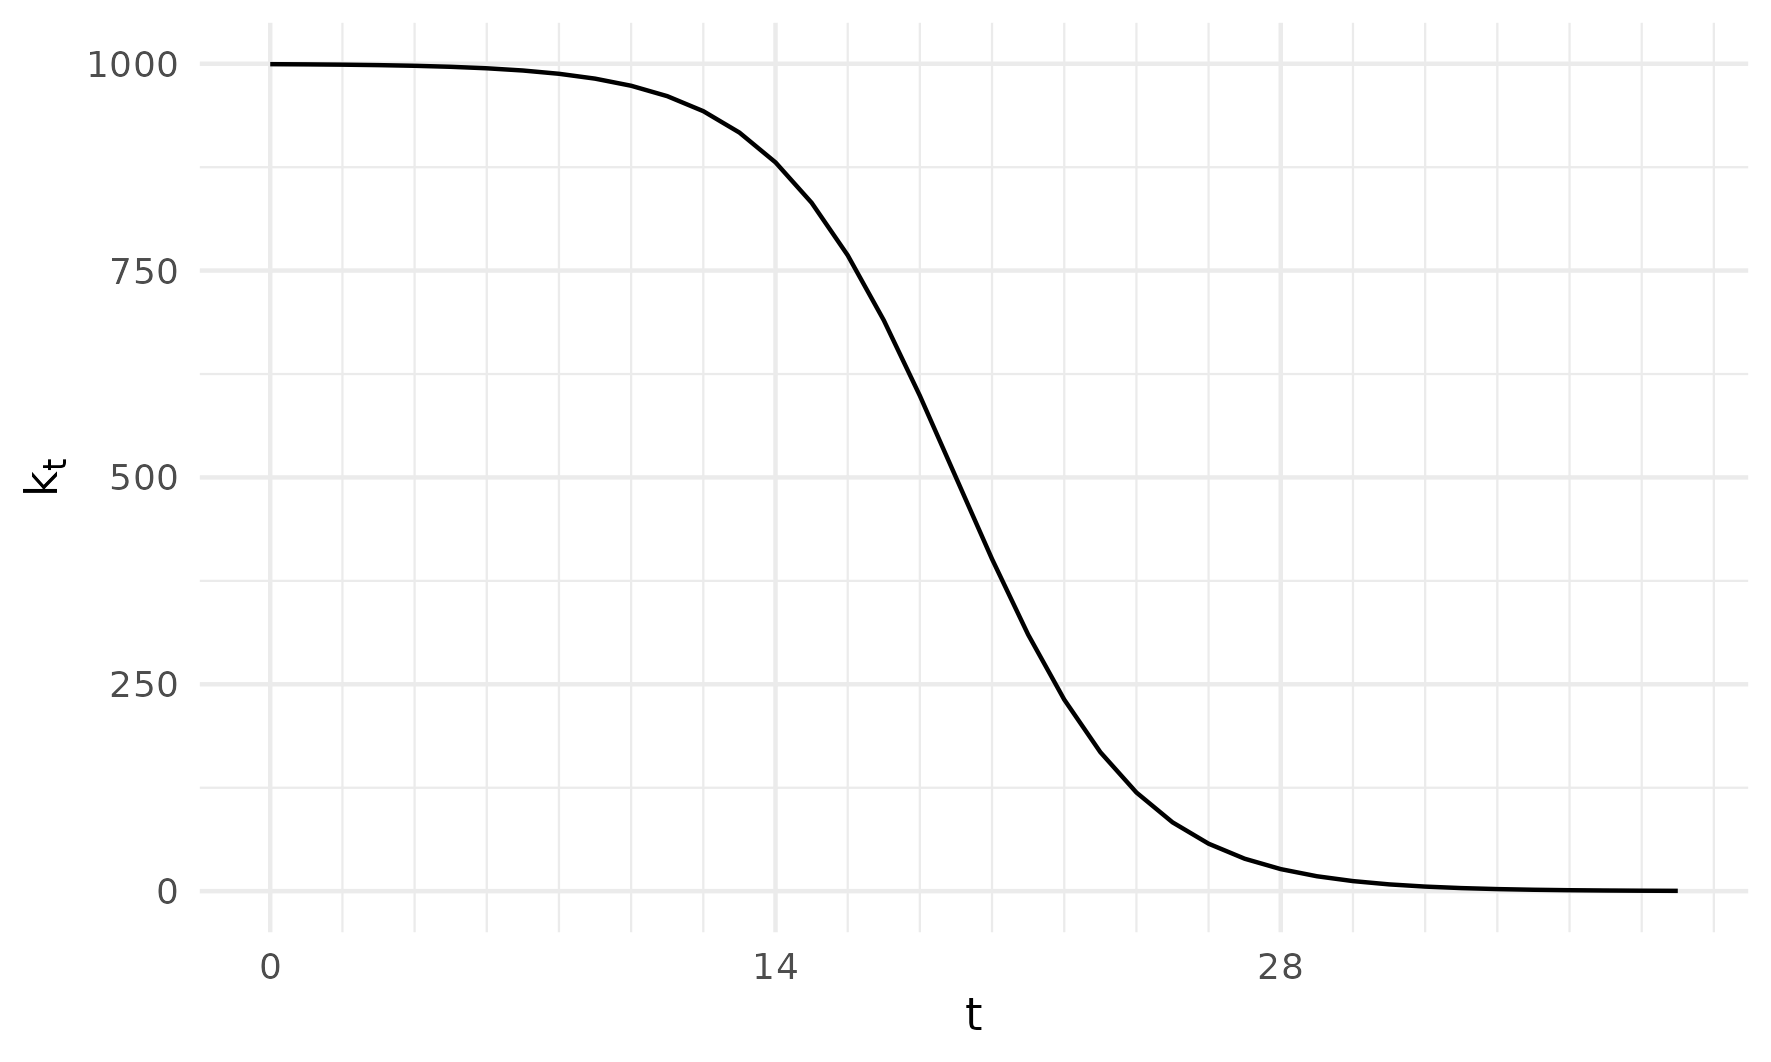
\includegraphics{cis-perfect-testing/kt-prior}
  \caption{Function used for $k_t$. \label{perf-test:fig:kt}}
\end{figure}

\section{Simulation study}

\subsection{Setup}

I simulate a dataset of detected episodes that has the same characteristics as that in the CIS by the following procedure.
\begin{enumerate}
    \item Extract the test schedules for each individual who had at least one test during the period of interest.
    \item Draw an episode start time, $b_{j(i)}$ for each individual uniformly at random between 2nd July 2020 (100 days before the period where a detected episode would be included) and 6th December 2020 (the end of this period).
    \item Draw a duration of episode for each individual, $d_i$, based on a modification of previous estimates (see \cref{duration-ground-truth}). Then calculate the end of their infection episode, $e_{j(i)} = b_{j(i)} + d_i - 1$.
    \item Simulate the test results based on the test schedule, $b_{j(i)}$, and $e_{j(i)}$. Tests between $b_{j(i)}$ and $e_{j(i)}$ (inclusive) are positive with positive probability (see below). All tests outside this interval are negative.
    \item Discard episodes where there are no positive tests (\ie undetected episodes) and then apply the same inclusions/exclusions as in \cref{perf-test:sec:problem}.
    \item Of these remaining episodes, sample 4,800 to match the sample size of the true dataset. This is needed because in step 2 the entire cohort was infected, while in the real study only a (unknown) portion is infected.
    \item For this final set of episodes, calculate $(l_j^{(b)}, r_j^{b}, l_j^{(e)}, r_j^{(e)})$ by taking the day after the last negative prior to any positives, the first positive, the last positive, and the day before the negative following the last positive respectively.
\end{enumerate}

I simulate data under this model by, for each test in a detectable individual, calculating $\psens(t-b)$, where $t$ is the day of the test and $b$ is the day the episode began.
The result of the test is then a Bernoulli random variable, independent of all other considerations.
Adapting the simulation study to incorporate this test sensitivity is much more similar to the data (see purple histogram in \cref{imperf-test:fig:sim-single-pos}).
This model does not require low test sensitivities early in the infection, maintaining compatibility with the results in \cref{E-ATACCC}.

I simulate datasets under four conditions: a constant $\psens$ of 0.6, 0.8, or 1.0, or the varying test sensitivity model proposed at the end of \cref{imperf-test:sec:simulate}.
The simulation is otherwise unchanged from that in \cref{E-perf-test:sec:simulation-study}.
The number of single positive episodes in each of these conditions, compared to the number observed in the CIS data, is shown in \cref{imperf-test:fig:sim-single-pos}.

For each simulated dataset, I estimate the survival function using the likelihood proposed in \cref{imperf-test:sec:modelling} and assuming $\psens$ equals 0.6, 0.8, or 1.0.
If the dataset was simulated using a constant $\psens$, and that value of $\psens$ matches the value assumed during inference, I refer to $\psens$ as being correctly specified; otherwise I refer to it as misspecified.
However, there is still some misspecification of the model to false negatives owing to the simplifying assumptions made.
The amount that the simplifying assumptions are violated increases as $\psens$ decreases.

\subsection{Implementation}

Simulation was performed in R~4.2.0~\autocite{R-4-2-0} using tidyverse~2.0.0~\autocite{tidyverse} and targets~1.1.3~\autocite{targetsPackage}.

Inference was implemented in Stan via RStan~2.21.8~\autocite{rstan2-21-8} using default settings.
Convergence was assessed using Rhat and ESS as described in \cref{E-MCMC:sec:convergence}, and all runs checked for divergent transitions.

The prior on the total number of infections was centred on the true value with a dispersion parameter of 1.
This meant that the prior was very diffuse.

\subsection{Results}

When $\psens = 0.8$ and is correctly specified, the model recovers the true survival time well (see \cref{imperf-test:fig:constant-test-sensitivity}(B)).
The informative prior, in comparison to the vague prior, helps to overcome the misspecification due to the simplifying assumptions, moving the estimated survival function closer to its true survival time.
However, when $\psens = 0.6$, this is no longer the case (see \cref{imperf-test:fig:constant-test-sensitivity}(A)).
This is likely caused by too large a violation of the simplifying assumptions made in \cref{imperf-test:sec:modelling}.
\begin{figure}
  % \makebox[\textwidth][c]{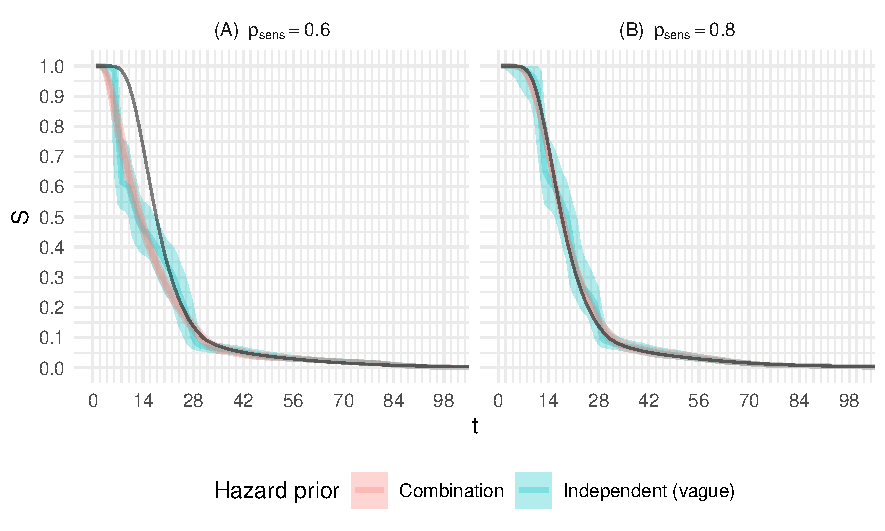
\includegraphics[width=1.2\textwidth]{cis-imperfect-testing/sim-constant-sensitivity}}
  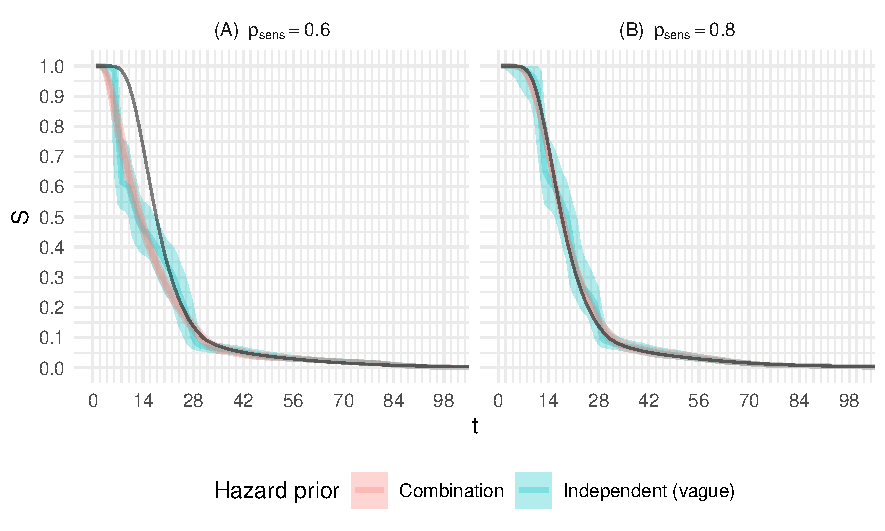
\includegraphics[width=\textwidth]{cis-imperfect-testing/sim-constant-sensitivity}
  \caption[Simulation study results with constant test sensitivity]{%
    Posterior (median and 95\% credible interval) of the survival time for the simulation study with a correctly specified test sensitivity.
    True survival time shown in black.
  }
  \label{imperf-test:fig:constant-test-sensitivity}
\end{figure}

Next, I considered the consequence of $\psens$ being misspecified, using the model combination prior; the better performing prior in the correctly specified case.
If the test sensitivity is misspecified, that is the assumed value for $p_\text{sens}$ in \cref{imperf-test:eq:pit-prime,imperf-test:eq:pit-prime} is different to the value used in the simulation, then the survival time will be biased (see \cref{imperf-test:fig:misspecified-test-sensitivity}).
If $\psens$ is misspecified and too low (see \cref{imperf-test:fig:misspecified-test-sensitivity}(A)), then the posterior estimate initially follows the true value but then separates.
The number of episodes inferred to have truly ended by the first negative is too high, and hence the survival time is overestimated.
This effect dominates over the opposing bias of overestimating the number of missed episodes.
The opposite occurs if the test sensitivity is assumed to be too high, although the posterior moves away from the truth earlier (see \cref{imperf-test:fig:misspecified-test-sensitivity}(C)).
\begin{figure}
  % \makebox[\textwidth][c]{
    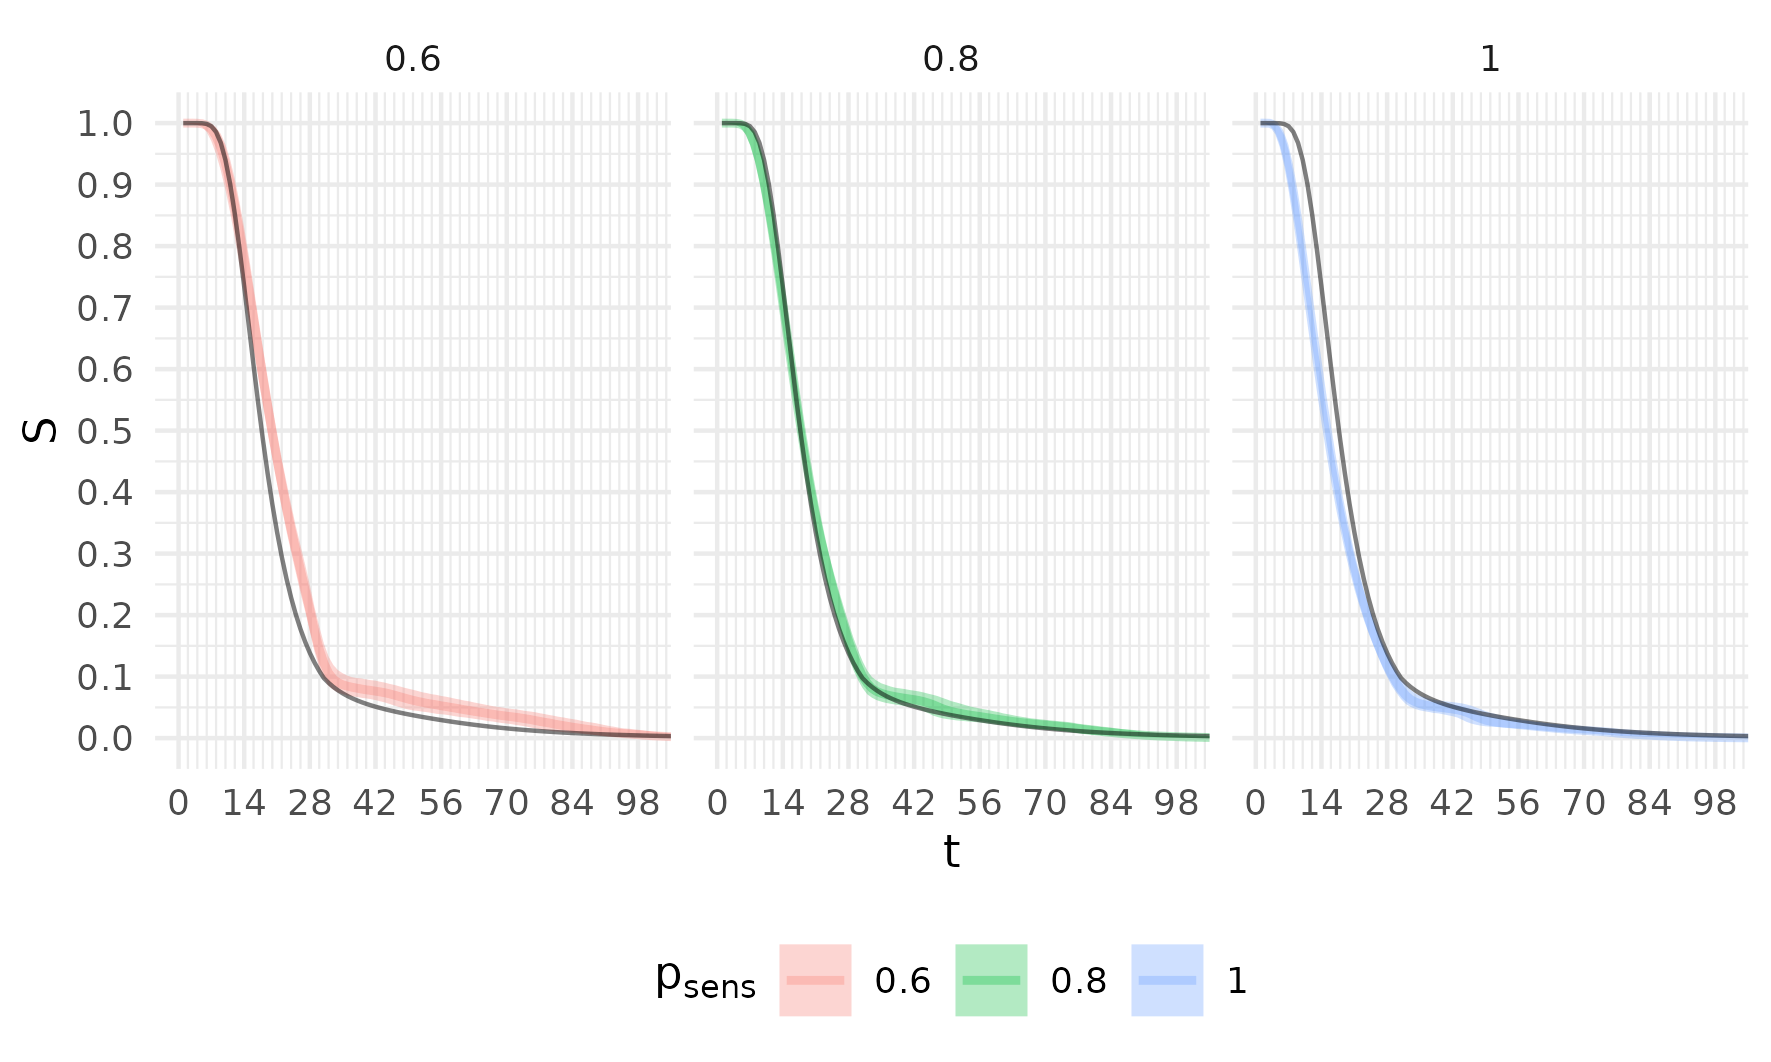
\includegraphics[width=\textwidth]{cis-imperfect-testing/sim-misspecified-sensitivity}
  \caption[Simulation study results with misspecified test sensitivity]{%
    Posterior (median and 95\% credible interval) of the survival time for the simulation study with a possibly misspecified test sensitivity.
    True survival time shown in black.
    All simulations use a constant test sensitivity of 0.8, but the inference procedure assumes different values, as per the key.
    Hence, (B) is correctly specified but (A) and (C) have misspecified $\psens$.
  }
  \label{imperf-test:fig:misspecified-test-sensitivity}
\end{figure}

The results when a varying test sensitivity (\cref{imperf-test:eq:variable-test-sensitivity}) is used for the simulation are similar to a constant 0.8 test sensitivity (see \cref{imperf-test:fig:variable-test-sensitivity}).
This suggests that the simplified model, with constant test sensitivity, is sufficient for recovering the true survival time.
Estimating the test sensitivity is not possible without a more complex model, as discussed in \cref{imperf-test:sec:discussion}.
Therefore, I will apply this model to the real CIS data in the next section.
\begin{figure}
  % \makebox[\textwidth][c]{
    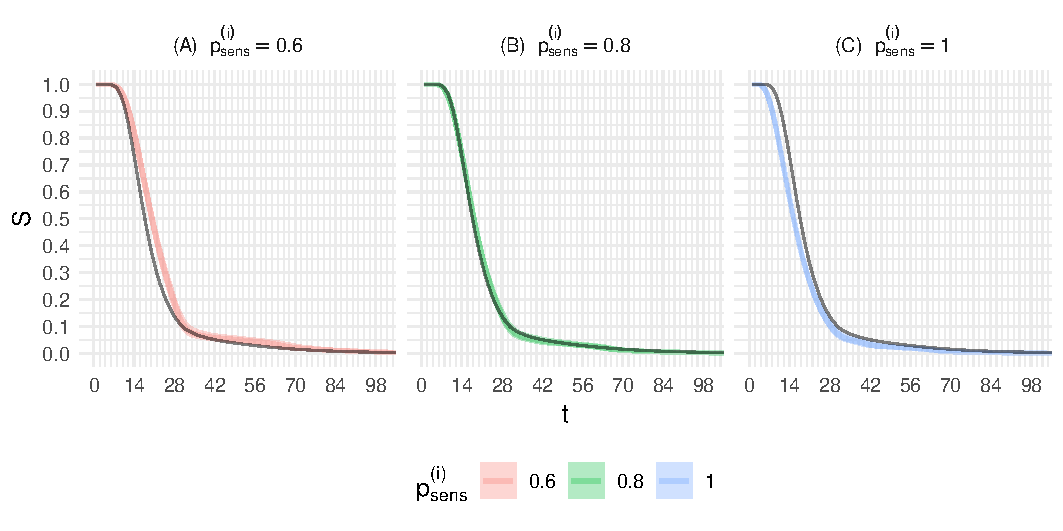
\includegraphics[width=\textwidth]{cis-imperfect-testing/sim-variable-sensitivity}
  \caption[Simulation study results with varying test sensitivity]{%
    Posterior (median and 95\% credible interval) of the survival time for the simulation study with a variable test sensitivity.
    Each panel shows the results of performing inference with a different assumed value for the test sensitivity.
    The posterior estimate using a model with a constant test sensitivity of 0.8 (B) is similar to the true value (black line).
  }
  \label{imperf-test:fig:variable-test-sensitivity}
\end{figure}

\section{Application}

In this section I apply the approach described in this chapter to the CIS episodes dataset I described in \cref{E-perf-test:sec:approach}.
This is the 4,800 CIS infection episodes first detected between 10th Oct 2020 and 6th Dec 2020 inclusive and have negatives bounding the start and end time of the episode.

Unlike in the simulation studies, an uninformative prior on $\ntot$ led to implausible estimates of the duration distribution.
The uninformative prior led to high posterior estimates of $\ntot$, and hence an implausibly large number of episodes with durations of less than five days.
Therefore, I based an informative prior for $\ntot$, $\ntot \sim \NBc(\mu, r)$ (as in \cref{E-perf-test:sec:model}, see \cref{E-distributions} for definition), using pre-existing estimates of the total number of infections to give $\mu\inform$ and $r\inform$.
\Textcite{birrellRTM2} estimated the total number of infections in England over the time period I consider, with posterior mean \numprint{4136368} and standard deviation \numprint{27932}.
% This model gives a posterior mean of \numprint{4136368} cumulative infections in England in the time period I consider, with a posterior standard deviation of \numprint{27932}~\citePersonalComms{Paul Birrell}.
\todo{Insert correct citation for RTM paper 2 once available}
Approximating this distribution as a negative binomial and scaling the mean to the size of the CIS cohort gives the prior $\mu\inform = 25132$ and $r\inform = 22047)$.

With this prior, the model produces plausible estimates of the duration distribution (see \cref{imperf-test:fig:cis-estimates}).
This estimate (blue) has more long episodes than the estimate in \cref{E-ATACCC} (red).

The qualitative increase in long episodes is robust to the choice of prior for $\ntot$, the assumed value for $\psens$ (see \cref{imperf-test:fig:cis-sensitivity}), and the choice of prior for the hazards, $\lambda_t$ (see \cref{E-perf-test:sec:parameters-priors}).
However, the survival proportion over the first 4 weeks is sensitive to these choices.
The estimate using a test sensitivity of 0.8 and $\NBc(\mu\inform, r\inform)$ give a median survival time most similar to that of \cref{E-ATACCC}.
\begin{figure}
  \centering 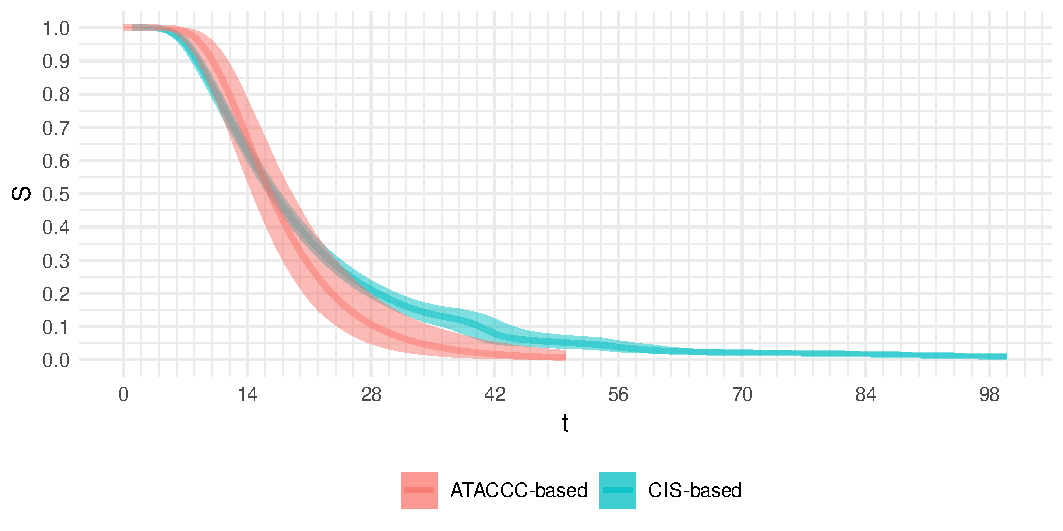
\includegraphics{cis-imperfect-testing/CIS_final}
  \caption{Duration estimates using CIS and ATACCC data}
  \label{imperf-test:fig:cis-estimates}
\end{figure}
\begin{figure}
  \vspace{-2.5cm}
  \makebox[\textwidth][c]{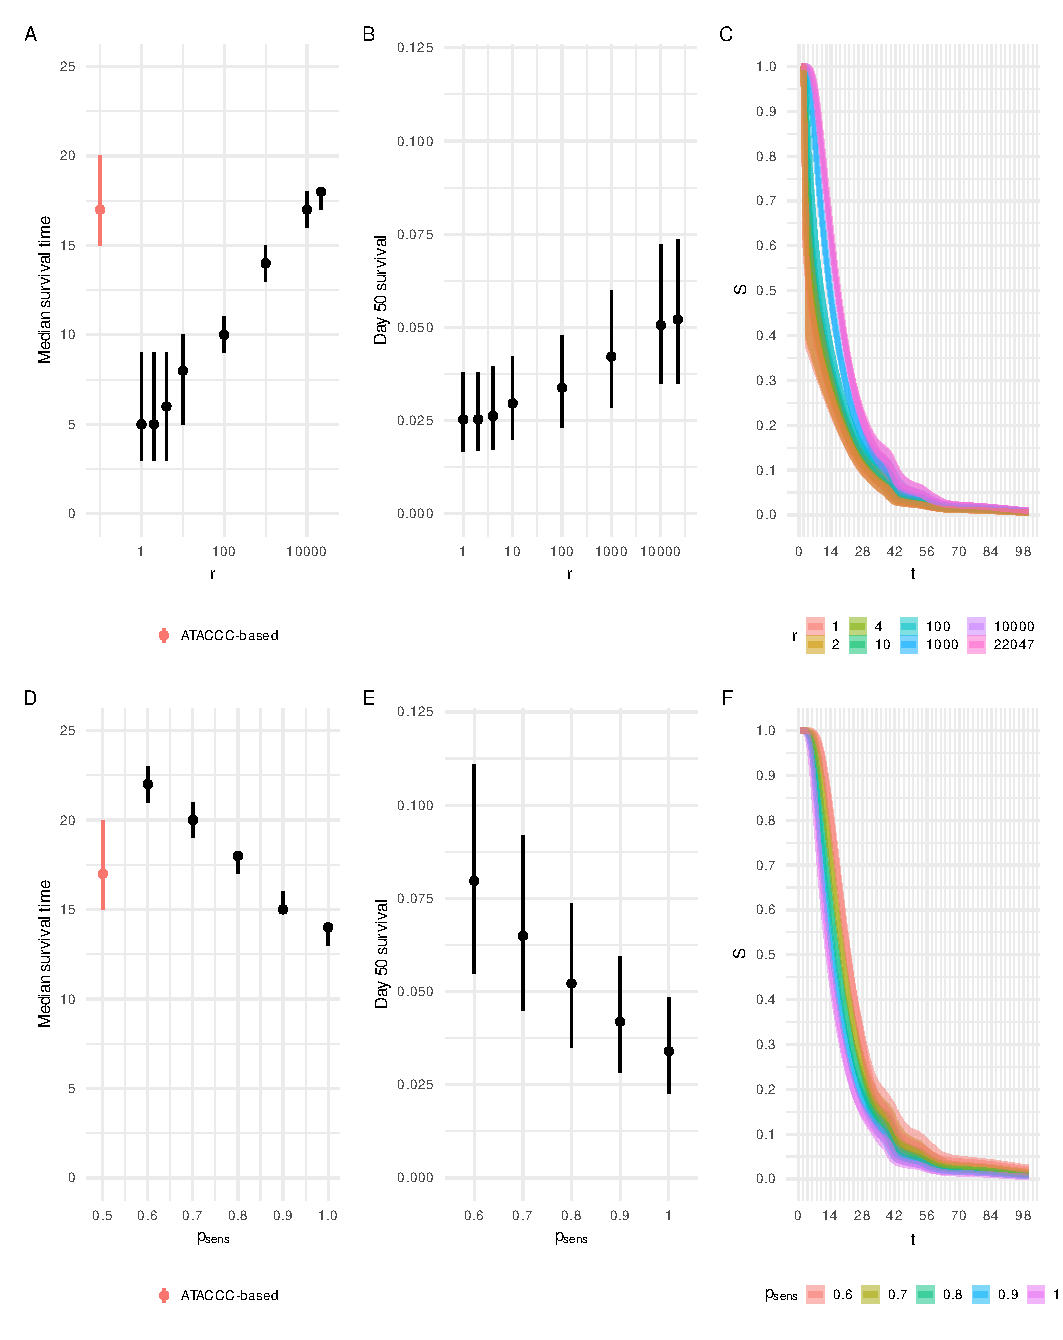
\includegraphics{cis-imperfect-testing/CIS_vary}}
  \caption{%
    (A-C) Sensitivity of CIS estimates to the value of $r$, the dispersion of the prior for $\ntot$ (a larger $r$ means a more informative prior) when $\psens = 0.8$.
    (D-F) Sensitivity of CIS estimates to the value of $\psens$ when $r = r\inform$.
    A and D: median survival time, in comparison to the ATACCC-based estimate of \cref{E-ATACCC} (shown in red).
    B and E: survival at day 50, $S_\theta(50)$.
    C and F: full survival curves out to day 100.
  }
  \label{imperf-test:fig:cis-sensitivity}
  \todo[inline]{Optional improvement: Could highlight the "preferred" model which exists in both rows and is the one used subsequently, and/or include ATACCC in the far-right hand column}
\end{figure}

The the estimates are most sensitive to the choice of $r$, the strength of the prior on $\ntot$.
A very weak, almost uninformative, prior on this quantity causes the posterior estimate to be much higher than the estimate from \textcite{birrellRTM2}.
When increasing the prior's strength, the posterior estimate moves towards the prior smoothly, as expected (see \cref{imperf-test:fig:ntot}).
As discussed previously, the \cref{E-ATACCC} estimates are reliable for the first 2--3 weeks, notably including the median time.
The median using $r\inform$ matched \cref{E-ATACCC}'s median estimate and is a principled choice because it is based directly on the prior work \textcite{birrellRTM2}.
Therefore, I use this estimate in the application to the CIS data.
\begin{figure}
  \centering 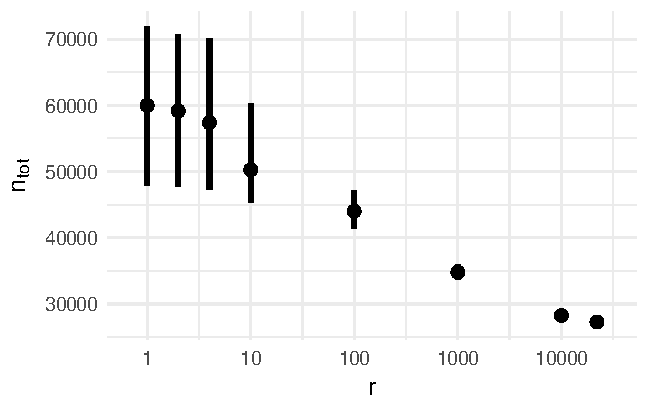
\includegraphics{cis-imperfect-testing/CIS_ntot}
  \caption{How the posterior estimate of $\ntot$ changes with the value of $r$ in the prior on $\ntot$.}
  \label{imperf-test:fig:ntot}
\end{figure}

\section{Discussion}

In this chapter, I developed a novel method to incorporate false negatives into the survival analysis of \cref{E-perf-test}.
I then applied this method to the CIS data, estimating the tail of the duration distribution without the strong model assumptions and extrapolation in \cref{E-ATACCC}.
The qualitative features of the estimated distribution are robust to the assumed value for $\psens$, and the choice of prior for $\lambda$, although the quantitative details are not.
The estimates of the tail, the primary purpose of this chapter, are in addition somewhat robust to the choice of prior for $\ntot$.
However, the rest of the distribution is sensitive to this choice.

An informative prior on $\ntot$ is required is for the bulk of the distribution to agree with those in \cref{E-ATACCC} and the wider literature.
In the simulation study, the uninformative prior on $\ntot$ performed well, even when the test sensitivity was misspecified.
A possible explanation is that the true changes in the test sensitivity is significantly different to the function in \cref{imperf-test:eq:variable-test-sensitivity}.
In particular, the test sensitivity for long episodes may become much lower than 50\%.
This allows many more episodes to be missed than the model assumes, and hence a higher $\ntot$ is required to explain the data.
Furthermore, it violates assumptions made in \cref{imperf-test:sec:modelling}; this is similar to when the simulating using a too low test sensitivity.
Violating these assumptions would lead to unpredictable inference results, perhaps those seen here.

Ideally, the test sensitivity would be estimated from the data.
However, this would require incorporating time-varying test sensitivity into the likelihood.
If the current model, with a constant $\psens$, is used then the estimate of $\psens$ would be heavily informed be intermittent negatives (the first, constant term in \cref{imperf-test:eq:pia-prime}).
These negatives will, in general, be further from the end of an episode than a randomly selected test.
Therefore, considering the viral dynamics from \cref{E-ATACCC}, the viral load will be higher and false negatives rarer.

Estimating the test sensitivity excluding intermittent negatives is not possible because \cref{imperf-test:eq:pia-prime-constant,imperf-test:eq:pit-prime} are both monotonically decreasing in $\psens$; therefore, the likelihood always favours $\psens = 0$ (\ie no true positives).
This aligns with the situation with singly interval censored, untruncated data, when stopping at the first observed time of the terminating event (which may be misclassified) means that the test sensitivity cannot be estimated~\autocite[e.g.]{titmanMisclassify}.

Estimating a time-varying $\psens$ with $S_\theta$ jointly may cause identifiability issues.
Previous studies have avoided issues by including external information (such as a prior giving the magnitude) on $\psens$, or test results from later follow-up~\autocite[and references therein]{piresIntervalMisclassify}.
However, these studies use a constant $\psens$.
Whether these methods are sufficient for the model to be identifiable with a time-varying $\psens$ needs further investigation.
A simple parametric form of the test sensitivity, such as that proposed by \textcite{brownBayesian}, may be sufficient to allow identifiability.
In any case, the likelihood, especially $p_{iu}'$, would be substantially complicated by such an addition which may greatly increase the computational cost of inference.

The assumption, made in \cref{E-perf-test}, was that the episode start times are independent.
However, because infections are the result of a counting process with intensity shared between individuals (see \cref{E-inc-prev:sec:infection-process}), this assumption is violated.
Prevalence was fairly constant over the period I chose, suggesting the same is true of the incidence.
Additionally, some simulations exploring the results of changing incidence suggested this would not have a large effect on the results (not shown).
\printbibliography[heading=bibintoc]

\appendix

\section{Defining episodes} \label{episodes}

\todo[inline]{This could be cut for a reference to \textcite{weiRisk}}

Positive test results need to be grouped into \emph{infection episodes}.
An infection episode is a series of positive tests that originate from a single transmission event.
I use a heuristic-based algorithm developed throughout the pandemic, and published within \textcite{weiRisk}; see that publication for full justification of the criteria.

The algorithm determines whether a new positive test, at time $t$, is part of the previous infection episode in the same individual.
If the individual has no previous positive tests, the new positive test is always the start of a new infection episode.
Otherwise, denote the first positive test associated with that previous infection episode as $t_p$, and the number of negative tests immediately prior to the test at $t$ as $n$.
The test at $t$, in the pre-Omicron era (prior to December 2021), is defined as the start of a new infection episode if any of the following apply.
\begin{enumerate}
  \item $n \geq 1$ and $t - t_p > 120$.
  \item $n \geq 2$ and $t - t_p > 90$.
  \item $n \geq 3$ and $t - t_p > 60$.
  \item $n \geq 4$.
  \item A complex heuristic based on the likely variant of the positive tests (see \textcite{weiRisk} for details). This heuristic rarely applied in the pre-Omicron era.
\end{enumerate}

A negative between two positive tests, when those positives are classed as part of the same infection episode, is known as an \emph{intermittent negative}.
Intermittent negatives are the clearest example of a false negative.
I will generally consider that intermittent negatives are uninformative on the duration of detectability, and hence exclude them from several analyses.

A sample of 500 randomly selected infection episodes (selected from the episodes used in the analyses in this thesis) have their test results shown in \cref{biology-data:fig:episodes}.
As can be seen, the number of tests within an episode, their length, and other characteristics vary greatly.
\begin{figure}
  \thisfloatpagestyle{empty}
  \vspace{-5cm}
  \makebox[\textwidth][c]{
\includegraphics[height=.7\paperheight]{biology-data/STATS13734/data_viz}}
  \caption[CIS infection episodes]{%
    500 randomly selected infection episodes.
    Shown are the negative tests before and after the outermost positive tests associated with the episode.
    Red dots are negative tests, green dots are positive tests, and blue dots are void tests (where the result could not be determined; excluded from other analyses).
  }
  \label{biology-data:fig:episodes}
\end{figure}

The crucial features of an infection episode are the start and end times of the infection.
Ignoring misclassified test results, latent start time of infection episode $j$, $B_j$, can be bounded as between the day after the last negative test, $l_j^{(b)}$, and the day of the first positive test, $r_j^{(b)}$.
Similarly, the latent end time of infection episode $i$, $E_j$, can be bounded as between the day of the last positive test, $l_j^{(e)}$, and the day before the following negative test, $r_j^{(e)}$.

\section{Duration distribution for simulation} \label{duration-ground-truth}

To generate the durations, an assumption is required for the distribution of the duration of positivity.
I base this assumption on the estimate from \cref{E-ATACCC} with an inflated tail to represent what is seen within CIS.
The tail is modified based on a previously unpublished analysis of CIS data, without accounting for several of the issues previously described.
Walker uses survival analysis to estimate the duration from CIS data.
The initiating event is assumed known as the time the episode was detected.
The final event is assumed interval censored between the time of the final positive test and the subsequent negative test, or right-censored if a negative test has not yet been observed.
A flexible, spline-based form is assumed for the baseline survival function~\autocite{roystonSTPM,roystonFlexible} with covariates introduced via proportional odds.
By not accounting for either the undetected infections or the interval censoring of the initiating event, this analysis has competing biases which makes them hard to interpret~\autocite{cisMethodsONS}.

% \todo[inline]{The following seems important to justify why we can't just use these estimates but is also basically an aside}
% We know of two biases introduced from this analysis.
% \enquote{There is a bias in estimating the clearance distribution because the analysis used to estimate how long a person stays positive only starts from their first positive test.
% Since (most) people will have become positive on an earlier day, this will bias the clearance curves downwards (making the estimates too short).
% However, there is another bias due to the survey missing positive episodes entirely if they are short.
% This means that our dataset has fewer short positive episodes than in the population as a whole, and that the sample used to run the survival analysis is biased towards people with longer positive episodes.
% This will bias the clearance curves upwards (making the estimates too long).}~\autocite{cisMethodsONS}.

To form the duration distribution used in the simulation, we combine the two estimates.
The first 30 days of the distribution is proportional to the ATACCC estimate, with the rest proportional to this CIS-based estimates.
Denote by $f_A(t)$ the distribution function estimated in \cref{E-ATACCC} and $f_C(t)$ that from the CIS-based estimates just derived.
Then define:
$$
f_S'(t) = \begin{cases}
	f_A(t) &t \leq 30 \\
	f_C(t) &t > 30
\end{cases}
$$
Then the distribution used in the simulation is the normalised version of this: $f_S(t) = f'_S(t)/\sum_i f_S'(i)$.
These curves and the combined curve are compared in \cref{perf-test:fig:duration-dist}.
Individual $i$'s duration of positivity, $D_i$, is then an independent draw from this distribution.
\begin{figure}
  \centering 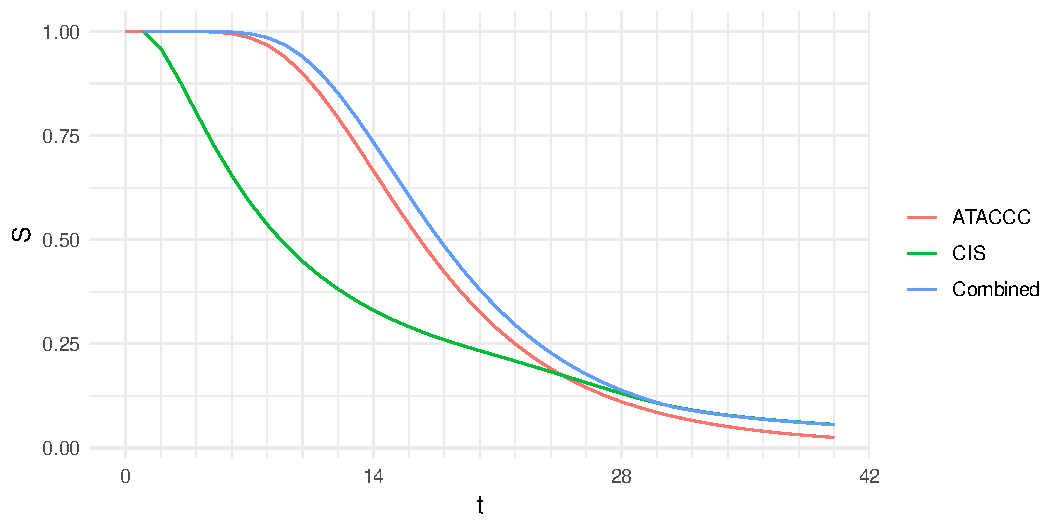
\includegraphics{cis-perfect-testing/input-duration-dists}
  \caption[Comparison of duration distributions]{Comparison of the duration distribution used for the simulation. ATACCC is the posterior mean from \cref{E-ATACCC}'s analysis, CIS is Sarah Walker's analysis, and Combined is the combination of these used for the simulation. See main text for details of each analysis. \label{perf-test:fig:duration-dist}}
\end{figure}



\end{document}

